%2multibyte Version: 5.50.0.2960 CodePage: 65001
%\input{tcilatex}

\documentclass[11pt]{article}
\usepackage{eurosym}
\usepackage[usenames,dvipsnames]{color}
\usepackage{graphicx}
\usepackage{amsfonts,amsthm,amssymb,amsmath}
\usepackage{booktabs}
\usepackage{enumitem}
\usepackage{multicol}
\usepackage{multirow}
\usepackage{longtable}
\usepackage{rotating}
\usepackage[maxfloats=30]{morefloats}
\usepackage[margin=1in]{geometry}
\usepackage{color}
\usepackage[center]{caption}
\usepackage{pdflscape}
\usepackage{placeins}
\usepackage{longtable}
\usepackage{setspace}
\usepackage{float}
\usepackage{pgffor}
\usepackage{calc}
\usepackage{graphics}
\usepackage{array}
\usepackage{comment}
\usepackage{bbm}
\usepackage{subcaption}
\usepackage{tikz}
\usepackage[backend=biber,style=apa,natbib=true]{biblatex}
\usepackage{xcolor}
\definecolor{darkred}{HTML}{8B0000}
\addbibresource{references.bib}
\usetikzlibrary{arrows.meta, positioning}
\usepackage{indentfirst}
\setlength{\parindent}{15pt}

\setcounter{MaxMatrixCols}{10}

\captionsetup{compatibility=false}
\captionsetup{
	font=normalsize,
	labelfont=normalfont,
	justification=centering
}

\usepackage{hyperref}
\hypersetup{
	colorlinks=true,
	linkcolor=Blue,
	urlcolor=Blue,
	citecolor=darkred
}

\DeclareCiteCommand{\cOne}
{\usebibmacro{prenote}}
{%
	\printtext[bibhyperref]{\textcolor{darkred}{\printnames{labelname}}}%
	\textcolor{black}{, }%
	\printtext[bibhyperref]{\textcolor{darkred}{\printfield{year}}}%
}
{\multicitedelim}
{\usebibmacro{postnote}}


\DeclareCiteCommand{\cTwo} % Author (Year) (paréntesis negros, con espacio)
{\usebibmacro{prenote}}
{%
	\printtext[bibhyperref]{\textcolor{darkred}{\printnames{labelname}}}%
	\addspace
	\textcolor{black}{(}%
	\printtext[bibhyperref]{\textcolor{darkred}{\printfield{year}}}%
	\textcolor{black}{)}%
}
{\multicitedelim}
{\usebibmacro{postnote}}

% Shorter aliases
\newcommand{\aaa}[1]{\cOne{#1}} % produces: Author, Year
\newcommand{\bbb}[1]{\cTwo{#1}} % produces: Author (Year)


\newcolumntype{H}{>{\setbox0=\hbox\bgroup}c<{\egroup}@{}}
\geometry{left=0.9in,right=0.9in,top=0.8in,bottom=0.8in}
\makeatletter
\newcommand*\ExpandableInput[1]{\@@input#1 }
\makeatother
\edef\savet{./3tables/v18}
\edef\savef{./2figures/v18}
\setcounter{tocdepth}{4}
\setcounter{secnumdepth}{4}
\newcommand\defComment[2]{\expandafter\def\csname Comment#1\endcsname{#2}}
\newcommand\CommentText[1]{\csname Comment#1\endcsname}

\begin{document}

\begin{titlepage}
	\centering
	\vspace*{-1cm}
	
\includegraphics[width=0.5\textwidth]{logo_UdeSA.png}\par\vspace{1cm}
	
	{\Large \textbf{Universidad de San Andrés} \par}
	\vspace{2mm}
	{\large Departamento de Economía \par}
	{\large Maestría en Economía \par}
	
	\vspace{2.2cm}
	
	{\LARGE \textbf{Democracy Does Cause Happiness} \par}
	
	\vspace{3cm}
	
	{\Large \textbf{Martin Iñaki Loriente} \par}
	{\normalsize 43170387}
	
	\vspace{1.6cm}
	
	{\large \textbf{Mentor}: Cevat Giray Aksoy}
	
	\vfill
	
	{\large 15 de Noviembre, 2025}
	
\end{titlepage}
	
\renewcommand\thefootnote{\fnsymbol{footnote}}
\begin{titlepage}
	
	\title{\textbf{Democracy Does Cause Happiness}\footnote{This work owes a great debt to the guidance and support of Cevat Giray Aksoy and Carlos Molina. Their mentorship, expertise, and constructive feedback have been instrumental in shaping the direction and quality of the research. Special acknowledgment goes to Christian Ruzzier, Martin Rossi and Nicolás Ajzenman, who served as members of the jury. Any remaining errors or shortcomings are solely the responsibility of the author.}}
	
	\normalsize
	
	\bigskip
	
	\renewcommand{\thefootnote}{\arabic{footnote}}
	\addtocounter{footnote}{+2}
	
	\bigskip
	
	\author{\Large{Martin Iñaki Loriente}\thanks{Universidad de San Andrés. Email: mloriente@udesa.edu.ar}\qquad \vspace{5mm}}
	
	\vspace{5mm}
	
	\date{\vspace{5mm} December 2025}
	
	\singlespacing
	\clearpage\maketitle
	\thispagestyle{empty}
	
	\vspace{3mm}
	
	\begin{abstract}
		 This paper provides causal evidence that democracy enhances individual well-being. Drawing on harmonized micro data from more than 100 countries and exploiting variation across birth cohorts and survey waves, the analysis shows that greater exposure to democratic institutions leads individuals to report higher income, better health, greater personal autonomy, higher life satisfaction, and greater subjective happiness. Building on recent literature documenting the effects of democratic transitions on economic growth, we shift the focus from national aggregates to individual-level outcomes to examine how democracy shapes personal welfare. The effects remain robust across alternative model specifications, clustering approaches, estimation strategies, sub samples, and a wide range of additional checks. The temporal dynamics further support our interpretation, as exposure during impressionable years plays a critical role. Mechanism analyses indicate that institutional performance is central: countries with stronger economic performance, greater transparency, higher state capacity, and more redistribution exhibit substantially larger effects, typically between 1.5 and 3 times those observed in lower-performing democracies.
		\begin{center}
			\hspace{-0.5cm}\textbf{Keywords:} democracy, happiness, health, income, autonomy, satisfaction, well-being. \\
			\hspace{-8.558cm}\textbf{JEL:} I31, O43, P16. 
		\end{center}
	\end{abstract}
	
\end{titlepage}


\spacing{1.35}
\newpage\clearpage

\section{Introduction}\label{Introduction}

“The secret of happiness is freedom, and the secret of freedom is courage.” Thucydides, History of the Peloponnesian War
\vspace*{0.5cm}

Do democratic institutions make people’s lives better? While economic growth is often regarded as the primary engine of improved living standards, democracy may have contributed to human well-being through channels that transcend material prosperity (\aaa{Haller2006}). By expanding political freedoms, fostering social stability, and strengthening individual autonomy, democratic institutions may have enhanced life satisfaction in ways that growth alone cannot achieve. For instance, \bbb{Kudamatsu2012} finds that democratization in sub-Saharan Africa was followed by a significant reduction in infant mortality, primarily through improved public health services rather than increased affluence. Understanding how democracy shapes both objective and subjective dimensions of well-being has therefore become essential for evaluating the broader benefits of democratic governance and informing institutional reform. Yet despite extensive debate, empirical evidence remains limited and fragmented. This paper aims to provide causal evidence on how democracy affects the different dimensions of well-being.

Whether democracy improves well-being primarily through economic growth has long remained an open question. If its effects operate only by raising incomes, then the value of democracy would depend on the extent to which economic gains translate into life satisfaction. Empirical evidence remains mixed. While income contributes to happiness (\aaa{Blanchflower2004}; \aaa{BenAfia2019}), marginal gains decline at higher levels (\aaa{Clark2014}), and classic sociological perspectives have questioned the durability of material progress as a source of happiness. The Easterlin Paradox (\aaa{Easterlin1974}; \aaa{DiTella2008}) shows that increases in national income do not necessarily yield long-term improvements in well-being, as inequality, social comparisons, and unemployment often offset temporary income gains (\aaa{Knight2011}; \aaa{Clark2016}; \aaa{Davies2011}). \bbb{Durkheim1893}, as interpreted by \bbb{Liagouras2019}, argued that intensified competition and rising aspirations may offset the psychological benefits of economic advancement. Taken together, these findings imply that economic progress accounts for only part of subjective well-being.

Consequently, a broader perspective on the determinants of happiness has emerged. Research highlights employment stability, political freedom, health, social trust, and community life as key drivers of well-being (\aaa{Deaton2008}; \aaa{Kahneman2004}; \aaa{Diener2012}). Social capital, in particular, provides a lasting foundation for life satisfaction (\aaa{Bartolini2014}). Institutional and cultural conditions have also been shown to shape well-being in ways that economic growth alone cannot capture (\aaa{Vemuri2006}; \aaa{Abdallah2008}; \aaa{OECD2011}; \aaa{OConnor2017}). This literature suggests that although growth contributes to well-being, its long-term impact is limited by inequality, social comparison, and non-material factors.

Recent evidence further indicates that public misperceptions about the benefits of democracy can help sustain support for authoritarian regimes. \bbb{Acemoglu2024} show that in Turkey, correcting such misperceptions about democracy and media freedom significantly increased support for opposition candidates. Complementary evidence from \bbb{Acemoglu2023} demonstrates that democracies can also cultivate their own legitimacy: individuals with longer exposure to successful democratic institutions display stronger support for democracy itself, particularly when such regimes deliver economic growth, stability, and good governance. Also, democracy has now been in retreat globally for almost two decades, according to recent assessments (\aaa{Repucci2021}).

These insights have renewed interest in democracy as an independent determinant of well-being. If economic growth explains only part of the story, democratic institutions may improve people’s lives directly by expanding freedoms, strengthening social stability, promoting health, and fostering individual agency. Empirical studies associate democracy with higher material welfare and greater life satisfaction, indicating that institutional environments play an independent role in shaping human flourishing.

Figure \ref{figure1} summarizes the conceptual framework that guides this analysis and illustrates both the economic and non-economic channels through which democracy may influence well-being. On the economic side, democratic institutions have been shown to stimulate growth by encouraging market-oriented reforms, reinforcing the rule of law, and reducing political instability (\aaa{Acemoglu2019}). These reforms promote investment, human capital accumulation, and job creation, thereby improving material living standards. At the same time, the redistributive effects of democracy are far from uniform. Evidence from \bbb{Acemoglu2015} indicates that although democratization raises fiscal capacity and schooling, it does not systematically reduce inequality, as outcomes depend on structural conditions and institutional capture. However, the effects of democracy extend beyond growth itself, since institutional quality also determines access to public goods, health services, and personal freedoms. Together, these mechanisms suggest that democracy enhances well-being both directly and indirectly, rather than solely through higher income.

A central non-economic mechanism is the expansion of personal autonomy. By safeguarding civil liberties, protecting property rights, and supporting open competition, democratic regimes enhance individuals’ control over their economic and social environments (\aaa{Kline2013}). Although higher income may facilitate greater independence, autonomy has been shown to exert an independent and lasting influence on life satisfaction. Individuals value the freedom to choose, participate, and shape their own trajectories, aspects that contribute to happiness regardless of material conditions (\aaa{Maestas2018}; \aaa{Bloom2015}; \aaa{Aksoy2022}). In this sense, democracy promotes well-being by expanding individual capabilities and civic agency rather than merely increasing economic output.

Beyond autonomy, democracy also strengthens the interaction between material and non-material dimensions of welfare. Economic reforms under democratic governance, such as trade liberalization or fiscal expansion, can promote entrepreneurship and financial independence (\aaa{Qin2024}; \aaa{Cesarini2017}) while simultaneously improving public health. These interrelated effects form a virtuous cycle in which healthier individuals tend to be more productive and earn higher incomes, while greater income supports better health outcomes and enhanced autonomy (\aaa{Oswald2006}). Democratic institutions amplify this cycle by enabling economic and social progress to reinforce one another. Consistent with this mechanism, \bbb{Baicker2019} provide evidence from the Oregon Health Insurance Experiment showing that improved access to health care can enhance individual autonomy and civic participation. Similar evidence from longitudinal studies shows that health conditions have a persistent and substantial impact on life satisfaction, often comparable to that of income (\aaa{Pagan2011}; \aaa{Powdthavee2017}). In sum, democracy has enhanced well-being through interdependent mechanisms. It has supported economic prosperity by fostering reform and stability, while also strengthening freedom, health, and agency. This framework has clarified how democratic governance improves individual lives and informs the empirical analysis that follows.

The timing of exposure to democratic institutions is crucial for understanding their impact on well-being. The impressionable years hypothesis argues that experiences during early adulthood leave lasting imprints on individuals’ values, attitudes, and expectations (\aaa{Krosnick1989}). This idea is supported by evidence showing that exposure to specific institutional environments between ages 18 and 25 shapes long-term beliefs and behaviors (\aaa{Dinas2013}; \aaa{Aksoy2020}; \aaa{Navajas2020}; \aaa{Cotofan2020}). Consistent with this view, our findings indicate that exposure to democracy during this formative period is strongly associated with greater autonomy and higher life satisfaction later in life (along other well-being results, including income, health and happiness). These results align with the capabilities approach from \bbb{Sen1999}, which emphasizes the role of substantive freedoms in enabling individuals to pursue lives they value. Democratic environments therefore contribute not only to material prosperity but also to the development of enduring preferences and capabilities that sustain well-being throughout the life course.

All this evidence indicates that although economic growth has remained an important driver of welfare, its contribution to well-being has been constrained by inequality, rising aspirations, and social comparisons. Democratic institutions, by contrast, have enhanced welfare through both material and non-material channels, with particularly strong effects when exposure has occurred during impressionable years. This perspective has provided a clearer understanding of how democracy has improved multiple dimensions of human well-being.

To establish causality, the analysis has combined harmonized microdata from more than one hundred countries with robust identification strategies, including instrumental variable estimation, alternative fixed effects structures, extensive robustness checks, and placebo exercises. Similar patterns have been obtained in the immigrant subsample from EVS, for whom democratic exposure during impressionable years has been defined in the country of birth. Across all specifications, greater exposure to democratic institutions has consistently produced positive and statistically significant effects on individual well-being, providing causal evidence that democracy has improved people’s lives.



\vspace*{0.5cm}
\section{Data and Empirical Strategy}\label{Data and Empirical Strategy}
\subsection{Data}\label{Data}
\vspace*{0cm}

The analysis leverages rich cross-country and cross-cohort variation to examine how democratic institutions shape individual well-being. A harmonized panel combining institutional and survey-based microdata is assembled to track changes in democracy and subjective outcomes over time and across birth cohorts. Differential exposure to democracy across countries and cohorts serves as a quasi-experimental source of variation, under the assumption that, conditional on fixed effects and covariates, trends in well-being would have evolved similarly in the absence of democratization.

A key input to the empirical strategy is the measurement of democracy. The Varieties of Democracy (V-Dem) dataset is used, as it provides the most comprehensive and fine-grained indicators of political institutions currently available (\aaa{Coppedge2024}; \aaa{Pemstein2024}). V-Dem covers 201 countries from 1789 to 2023 and conceptualizes democracy along five core dimensions: electoral, liberal, participatory, deliberative, and egalitarian. These variables jointly capture both formal institutions and de facto practices. Each dimension is constructed from multiple factual and evaluative indicators coded by nearly 3,000 country experts following standardized protocols.

To construct a continuous measure of democracy, these five dimensions are aggregated into a country–year index, $C_{ct} \in [0,1]$. This measure varies both across countries and within countries over time, allowing the exploitation of institutional change at different stages of development and state formation. The multidimensional structure of V-Dem helps address several limitations of earlier datasets, such as low reliability in binary indicators (\aaa{Elkins2000}), attenuation bias and coder disagreement in continuous indices (\aaa{Pemstein2010}), and the lack of conceptual granularity in aggregated measures (\aaa{Claassen2020}). As a result, V-Dem has become the dominant source for empirical research on democratic institutions (\aaa{Luhrmann2017}; \aaa{Dahlum2019}; \aaa{Singh2019}).

This preferred continuous measure is complemented with a dichotomous democracy index, $D_{ct} \in \{0,1\}$, which captures the extensive margin of regime change and serves as a robustness check for potential classification disputes near the democracy threshold. This binary indicator is not designed to replace the continuous metric or to address attenuation bias already accounted for in V-Dem. Rather, it isolates episodes where institutional change reflects a clear regime transition instead of incremental variation in institutional quality. It is constructed using a harmonized aggregation of the leading datasets in the institutional literature (\aaa{Cheibub2010}; \aaa{Boix2018}; \aaa{Acemoglu2019}; \aaa{FreedomHouse2021}; \aaa{Marshall2018}), and a country is coded as democratic only when multiple sources agree in their classification. This consensus-based approach promotes conceptual consistency and reduces false positives in borderline cases. By jointly employing a continuous (V-Dem) and a dichotomous measure, both the intensive margin of democratic quality and the extensive margin of regime type are captured, allowing an examination of whether the effects of democracy on well-being are driven by institutional depth or by the existence of democratic rule itself.

Our outcomes are drawn from the Integrated Values Surveys (IVS), which harmonize the European Values Study and the World Values Survey into a single globally comparable dataset (\aaa{EVS2022}; \aaa{Haerpfer2022}). These large-scale surveys provide consistent information on attitudes, values, and self-reported well-being for individuals across 103 countries from 1981 to 2022, although coverage varies by wave. This structure enables us to link variation in exposure to democracy across both cohorts and countries to multiple dimensions of well-being, including income, health, personal autonomy, life satisfaction, and happiness. 

Democratic exposure during impressionable years and over the life cycle exhibits substantial variation not only across countries but also within countries across birth cohorts, providing the primary source of identification in our empirical strategy. Appendix Figure \ref{af1}a displays the time series of the democracy index for each of the 103 countries in our sample and highlights four cases for illustration: Argentina, Turkey, South Korea, and the United States. Appendix Figure \ref{af1}b presents variation in exposure to democracy during the impressionable years, defined as ages 18 to 25, across cohorts in all countries while again emphasizing those selected cases. As the figures show, exposure to democracy varies markedly both across countries and across cohorts within each country, and this rich cross-cohort and cross-country variation is precisely what our empirical design exploits.

To analyze how country-level institutional quality and economic performance condition the effects of democracy on individual well-being, several complementary country–year measures are incorporated. Real GDP growth is constructed using data from the Maddison Project (\aaa{Bolt2020}; \aaa{Bolt2020B}), the Penn World Tables (\aaa{Feenstra2015}), and World Bank national accounts (\aaa{WorldBank2023}), covering 188 countries and 18,760 country–year observations. Political corruption is measured using a V-Dem index based on expert assessments of the pervasiveness of political corruption, ranging from 0 to 1 for 177 countries and 28,024 country–year observations from 1789 to 2021. This measure is inverted to obtain a transparency indicator. State capacity is also measured using a V-Dem index reflecting the extent to which governments can effectively implement policy, capturing the administrative dimension of institutional quality. Finally, to analyze the redistributive effects of democracy, data from the World Inequality Database (\aaa{WID2025}) on the income share of the top 1 percent of the population are used, covering 184 countries and 9,377 country–year observations, with broader availability after 1980. From this series, a dichotomous indicator is constructed classifying each country–year according to whether top income shares are above or below their historical median, with lower concentration interpreted as greater redistributive performance. For details on the construction of inequality series, see the World Inequality Report (\aaa{Alvaredo2018}).

The European Social Survey provides high-quality microdata for a wide set of European countries, collected through uniform questionnaires, strict sampling protocols, and consistent fieldwork standards across waves. Its structure allows the construction of well-being measures that follow the same logic as in the IVS, making it well suited for a direct replication of the empirical approach. For this reason, the European Social Survey is also used as an additional dataset to validate the baseline findings (see \aaa{ESS2024}).

Appendix Tables \ref{at1} and \ref{at2} summarize the variables used in the analysis, including well-being outcomes and democratic exposure measures. The statistics reveal substantial variation both across and within countries over time, particularly in exposure to democracy across birth cohorts, which underpins our identification strategy. Appendix Table \ref{at3} documents the regional distribution of respondents, confirming that the sample provides broad global coverage and considerable heterogeneity within regions. 


\vspace*{0.5cm}
\subsection{Empirical Strategy}\label{EmpiricalStrategy}

The methodology of \bbb{Acemoglu2024} is followed to construct measures of exposure to democracy, capturing the accumulated number of years an individual has lived under a democratic regime within a given time window. Consequently, democracy is treated as a predetermined cumulative exposure with respect to the outcome, rather than as a contemporaneous measure. In addition, exposure is measured over specific age groups. Specifically, two complementary measures are computed:

\begin{enumerate}
	\item \textit{Lifetime Exposure to Democracy}, which sums the years lived under democracy from age 6 until the survey year, capturing the overall democratic environment experienced by the respondent.
	
	\item \textit{Exposure to Democracy during Ages 18--25}, focusing on the so-called “impressionable years”, when political and institutional experiences are thought to leave lasting effects. 
\end{enumerate}

These two complementary measures can be formally expressed as follows for an individual of age a in country c observed in survey year s:

\begin{equation}
	\label{1}
	\begin{aligned}
		\text{Exposure to Democracy}_{c,s,a} 
		&= \sum_{t=s-a+k}^{s} D_{c,t} \\[1em]
		\text{Exposure to Democracy 18--25}_{c,s,a} 
		&= \sum_{t = s-a+18}^{\,\,s-a+25} D_{c,t}
	\end{aligned}
\end{equation}

where $D_{c,t}$ is either our dichotomous or continuous measure of democracy for country c in year t. The summation is taken over the lifetime of an individual of age $a$, starting when the individual was $k$ years old and extending to the present year $s$. This measure represents an individual’s cumulative exposure to democracy. In the baseline specification, $k = 6$, capturing exposure from the typical start of compulsory schooling. Evidence reported in the online appendix shows that the results are not sensitive to this choice: alternative starting ages yield estimates that remain positive and statistically significant, with effect sizes of similar magnitude. The time window defining impressionable years is also shown to be robust to small changes.

To ensure consistency across specifications, the sample is restricted to observations with complete information on demographic characteristics, democracy exposure measures, and country-level controls. This harmonization guarantees that all estimates are based on the same underlying sample and that differences across tables are driven by model specifications rather than changes in sample composition. Because exposure during the impressionable years is only defined for individuals aged 25 or older, the sample used in those regressions naturally contains older respondents, yielding meaningful variation between lifetime and early-adulthood exposure. Immigrants are excluded from the main sample and analyzed separately later.

We estimate the following benchmark regression:
\begin{equation}
	\label{2}
	\text{Outcome}_{i,w,c,s,a} = \beta \text{Exposure to Democracy 18-25}_{c,s,a} + \gamma^{\prime}X_{i,w,c,s,a} + \varepsilon_{i,w,c,s,a} 
\end{equation}
where $\text{Outcome}_{i,w,c,s,a}$ is a measure of well-being for individual $i$, observed in survey wave $w$, country $c$, year of interview $s$, and age $a$. The key regressor, $\text{Exposure to Democracy 18-25}_{c,s,a}$, captures democratic exposure during impressionable years. Individual indices $i$ appear only in variables measured at the respondent level (outcomes, controls, and residuals). The main regressor, varies across country, survey year, and cohort but remains constant for all individuals sharing those characteristics, since it is computed as the national average level of democracy experienced between ages 18 and 25. An analogous specification is used to estimate the effect of lifetime exposure to democracy. In alternative specifications, the democracy measure is interacted with various success criteria to construct exposure to successful democracy. 

The vector $X_{i,w,c,s,a}$ includes individual-level controls, varying by specification. Our main specifications include the following fixed effects:
\begin{itemize}
	\item Specification 1: gender, town size, wave of the survey, age, language, sub-region, year of birth, country, and year of interview.
	\item Specification 2: gender, town size, wave of the survey, age, language, sub-region, fixed effects for region $\times$ year of interview, and country $\times$ wave of the survey.
\end{itemize}

Focus is placed on specification (1) for most of the analysis. Because age, birth cohort, and survey year are perfectly collinear, different combinations of fixed effects impose alternative normalizations in the APC space. The stability of the estimated democracy coefficient across these specifications confirms that identification is robust and not sensitive to the chosen normalization. Unless stated otherwise, all regressions use heteroskedasticity-robust standard errors clustered at the country and survey-year levels. Results remain largely unchanged across ten alternative specifications (Appendix Table \ref{at4}) and remain statistically significant when using ten different clustering definitions (Appendix Table \ref{at5}). Additional robustness evidence is reported in the online appendix. 

The \textit{Exposure to Successful Democracy} variable is computed by multiplying the democracy and success indicators for each year from age 6 to the year of the interview, and summing the resulting products. For example, consider a respondent to the World Value Survey 7 in the United States in 2020. If the individual lived in a successful democracy throughout the lifetime, as defined by the success criteria, and a dichotomous democracy measure is used, exposure corresponds to the total number of years from age 6 to 2020 in which both democracy and success equal one. The impressionable-years exposure to successful democracy is defined analogously, but restricted to that age window.

The analysis includes a model that separates exposure to successful democracy, unsuccessful democracy, and unsuccessful autocracy, leaving successful autocracy as the omitted category, where success is defined on the basis of economic performance, transparency, state capacity, and redistribution.

\begin{equation}
	\label{3}
	\begin{split}
		Outcome_{i,w,c,s,a} 
		= & \; \tilde{\beta}_{1} \, \text{Exposure to Successful Democracy}_{c,s,a} \\
		& + \tilde{\beta}_{2} \, \text{Exposure to Unsuccessful Democracy}_{c,s,a} \\
		& + \tilde{\beta}_{3} \, \text{Exposure to Unsuccessful Autocracy}_{c,s,a} 
		+ \tilde{\gamma}' X_{i,w,c,s,a} 
		+ \tilde{\varepsilon}_{i,w,c,s,a}
	\end{split}
\end{equation}

where the exposure variables are calculated separately for periods of successful and unsuccessful performance. Specifically,

\begin{equation}
	\label{4}
	\begin{aligned}
		\text{Exposure to Successful Democracy}_{c,s,a} 
		&= \sum_{t=s-a+k}^{s} D_{c,t} \times M_{c,t} \\[1em]
		\text{Exposure to Unsuccessful Democracy}_{c,s,a} 
		&= \sum_{t=s-a+k}^{s} D_{c,t} \times (1 - M_{c,t}) \\[1em]
		\text{Exposure to Unsuccessful Autocracy}_{c,s,a} 
		&= \sum_{t=s-a+k}^{s} (1 - D_{c,t}) \times (1 - M_{c,t}) \\[1em]
		\text{Exposure to Successful Democracy 18--25}_{c,s,a} 
		&= \sum_{t = s-a+18}^{\,\,s-a+25} D_{c,t} \times M_{c,t} \\[1em]
		\text{Exposure to Unsuccessful Democracy 18--25}_{c,s,a} 
		&= \sum_{t = s-a+18}^{\,\,s-a+25} D_{c,t} \times (1 - M_{c,t}) \\[1em]
		\text{Exposure to Unsuccessful Autocracy 18--25}_{c,s,a} 
		&= \sum_{t = s-a+18}^{\,\,s-a+25} (1 - D_{c,t}) \times (1 - M_{c,t}),
	\end{aligned}
\end{equation}

where $M_{c,t}$ is a dummy variable taking the value of one when country c is successful at time t according to the chosen criterion (e.g., economic expansion vs. recession).

For brevity, estimation focuses on equation \eqref{3} using exposure measures constructed from the continuous democracy index, which provides greater variation and typically yields larger estimates than the dichotomous measure depicted in the equation. Results based on the dichotomous democracy index, which allows a more straightforward interpretation and delivers estimates with similar signs and statistical significance, are reported in the online appendix. The key identifying assumption in both equations \eqref{2} and \eqref{3} is that, absent differences in exposure to democracy, well-being would follow similar trends across birth cohorts within a country, conditional on the full set of fixed effects included in the specification. To assess this assumption, evidence is provided showing that pre-birth exposure to either successful or overall democracy is uncorrelated with well-being, while estimates for exposure during impressionable years, lifetime exposure, and successful exposure diverge sharply from these pre-trends (Figure \ref{figure2} and Appendix Figures \ref{af2}-\ref{af6}).

In the regressions, the original survey weights are used and rescaled within each country-wave so that they sum to 1,000 observations. This procedure preserves the internal distribution of respondents within each country–wave while ensuring that all units contribute equally to the analysis, preventing countries with larger samples from dominating the results. Conceptually, this transformation is equivalent to the survey’s equilibrated weights, but applied at the country–wave level rather than globally. This approach enhances comparability without distorting the relative composition of the samples.

\vspace*{0.5cm}
\subsection{Variable Description}

Five key well-being variables are examined using data from the Integrated Values Survey (IVS), which combines the World Values Survey (WVS) and the European Values Survey (EVS).

\vspace*{0.5cm}
\begin{center}
	\large \textbf{Summary of Outcomes}
\end{center}

\begin{enumerate}[label={\arabic*.}]
	\item \textbf{Income}: $X047R\_EVS + X047R\_WVS$, available for EVS1, EVS2, EVS4, EVS5, WVS1–WVS7. It combines two recoded variables from EVS and WVS. In EVS, respondents indicate the income group of their household after taxes, ranging from 1 to 15. In WVS, respondents indicate their household's position on a 1–10 decile scale. The IVS harmonizes both into three categories: 1 = low, 2 = medium, 3 = high, covering more survey waves and reducing missing data.
	
	\item \textbf{Health}: $A009$, available for EVS1, EVS2, EVS4, EVS5, WVS1 to WVS7. Respondents rate their health from ``Very poor'' to ``Very good.'' This variable is converted into a binary measure: 0 = poor (Very poor, Poor, Fair), 1 = good (Good, Very good).

	\item \textbf{Autonomy}: Available for EVS1, EVS2, EVS4, EVS5, and WVS1 to WVS7. An index of individual autonomy is constructed based on three survey items: perceived freedom of choice and control over life ($A173$), importance of independence in child-rearing ($A029$), and rejection of obedience as a desirable child quality ($A042$). Each item is standardized, averaged, and rescaled to range from 1 to 2 as follows:
	\[
	\text{A} = \frac{z_{\text{childindepend}} + z_{\text{childobed}} + z_{\text{free}}}{3},
	\quad
	\text{autonomy} = \frac{\text{A} - \min(\text{A})}{\max(\text{A}) - \min(\text{A})} + 1
	\]
	Higher values indicate greater perceived personal autonomy and a stronger preference for individual independence over conformity.

	\item \textbf{Life Satisfaction}: $A170$, available for EVS1–EVS5, WVS1–WVS7. Respondents report overall life satisfaction on a 1–10 scale, where 1 = completely dissatisfied and 10 = completely satisfied.

	\item \textbf{Happiness}: A008, available for EVS1–EVS5, WVS1–WVS7. Respondents indicate their general happiness from “Not at all happy” to “Very happy.”
\end{enumerate}

\vspace*{0.5cm}
\begin{center}
\large \textbf{Summary of Measures for Success}
\end{center}

All success measures are binary, indicating whether a country-year observation meets a defined performance threshold.

\begin{enumerate}[label={\arabic*.}]
	\item \textbf{Growth}: 1 if the standardized country-year GDP per capita growth is not in the lower tail of the global distribution, defined as being no more than one standard deviation below the global mean; 0 otherwise. This threshold is intended to capture severe macroeconomic underperformance rather than above-average growth, thereby classifying all non-crisis episodes as successful. Alternative thresholds and continuous measures yield similar results. Sources: Maddison Project, World Bank, \bbb{UNSD2023}.
	
	\item \textbf{Transparency}: 1 if the standardized complement of country-year political corruption index is $\ge 0.5$ SD above the global mean; 0 otherwise. In this sense, it is a variable that defines the control of corruption. Source: V-Dem.
	
	\item \textbf{Capacity}: 1 if the standardized country-year state capacity is $\ge -1$ SD below the global mean; 0 otherwise. Source: V-Dem.
	
	\item \textbf{Redistribution}: 1 if the country-year top 1\% income share is below its historical median (redistributive success); 0 otherwise. Source: World Inequality Database (WID).
\end{enumerate}

Taken together, these five outcomes capture both more material (income, health) and subjective (life satisfaction, happiness, autonomy) dimensions of individual well-being. The success measures, by contrast, characterize country-level institutional performance and enable us to assess whether the well-being effects of democracy depend on the quality of governance. By interacting democratic exposure with growth, transparency, state capacity, and redistribution, we can distinguish whether democracy improves lives only when institutions function effectively, or whether its benefits extend even under unfavorable conditions. This structure provides a coherent empirical framework for identifying the causal impact of democracy on well-being across heterogeneous institutional environments.



\vspace*{0.5cm}
\section{Main Results}\label{Main}
\subsection{Exposure to Democracy and Well-Being}\label{Main1}

Table \ref{table1} present the estimated effects of exposure to democracy during early adulthood (18 to 25 years) and over the life cycle on income, health, autonomy, life satisfaction, and happiness. Across all outcomes and specifications, both the dichotomous and continuous measures of democracy yield positive and statistically significant coefficients, indicating a consistent improvement in well-being associated with democratic exposure. All outcomes are standardized to have mean zero and unit variance, so coefficients can be interpreted as standardized effects. We focus on the continuous index as our preferred measure because it captures variation in institutional quality, while the dichotomous measure is used to demonstrate robustness. A one-standard-deviation increase in exposure during early adulthood increases income by 0.081 standard deviations (0.120 for lifetime exposure), health by 0.085 (0.197), life satisfaction by 0.065 (0.159) and happiness by 0.067 (0.138). Autonomy displays similar effects for early-adulthood exposure (0.054) and lifetime exposure (0.057), suggesting that democratic institutions primarily shape agency during formative years. Lifetime exposure generally produces the largest effects, reflecting the cumulative impact of democratic institutions across the life course.

The timing of democratic exposure plays a central role in shaping long-term well-being. Tables \ref{table2} and \ref{table3} compare six age windows (2–9, 10–17, 18–25, 26–33, 34–41, and cumulative lifetime exposure) and show that exposure between ages 18 and 25 is the only period that consistently remains statistically significant across all specifications and outcomes. This robustness indicates that early adulthood is the most consequential phase for the internalization of democratic norms and the formation of long-run preferences. While later adulthood windows (26–33 and 34–41) also display positive and occasionally sizable effects, their significance is less systematic across outcomes. These results suggest that democratic exposure throughout life contributes to well-being, but the impressionable years interval exerts a uniquely persistent and central influence.

In the specification that includes both lifetime and impressionable years exposure, the lifetime coefficient captures the effect of democratic exposure accumulated across the life course outside the impressionable period, whereas the impressionable years coefficient isolates the additional effect of exposure specifically between ages 18 and 25. The estimates reveal heterogeneous temporal patterns across outcomes. For health, life satisfaction, and happiness, both coefficients are positive and statistically significant, indicating that democracy has exerted enduring effects over the life span while additionally generating an independent impact during early adulthood. In contrast, for income and autonomy, only the impressionable years exposure remains statistically significant in our data, suggesting that any benefits of democracy on these outcomes are largely concentrated in the formative period, with no additional evidence of effects from later exposures once early-adulthood exposure is accounted for.

Taken together, these findings provide consistent evidence that exposure to democratic institutions, particularly during early adulthood, has a robust and meaningful effect on well-being. The positive effects on life satisfaction and happiness appear to be plausibly mediated through improvements in income, health, and autonomy. These results underscore the importance of both the timing and quality of democratic exposure, demonstrating that institutional experiences have shaped both subjective and material dimensions of well-being over the life course.



\vspace*{0.5cm}
\subsection{Other Results}\label{Main2}

Our results suggest that, in our sample, the effects of democratic exposure do not fade over time; instead, they appear to persist and, for several outcomes, intensify across the life course. Table \ref{table4} demonstrates that the interaction between early-adulthood exposure and age is positive and statistically significant for health, happiness, and life satisfaction, indicating that the benefits of democracy compound as individuals grow older. For income and autonomy, the interaction is not statistically different from zero, indicating that we do not find evidence of age-related changes in these effects within our sample. The increasing effect on health is particularly meaningful because initial levels of self-reported health are high among young individuals, and the influence of democratic exposure becomes more salient as age-related health differences emerge. Overall, these findings indicate that exposure to democratic institutions during the impressionable years generates enduring and, in some cases, expanding gains in well-being throughout the life cycle.

Institutional quality enhances the effect of democracy on well-being, but democratic benefits extend even to societies with less developed institutions. Table \ref{table5} compares exposure during the impressionable years across four institutional regimes: Successful Democracy, Unsuccessful Democracy, Successful Autocracy (the omitted category), and Unsuccessful Autocracy. In each panel, “success” refers to favorable performance in economic growth, transparency, state capacity, or redistribution. Individuals exposed to successful democracies have consistently reported higher well-being than those exposed to successful autocracies, confirming that democracy generates distinctive advantages even when autocracies achieve comparable institutional outcomes. This framework has also made it possible to separate the combined effect of democracy and institutional success from the effect of democracy alone, since comparing successful and unsuccessful democracies isolates the independent contribution of democratic institutions.

The results have shown that favorable institutional conditions amplify democracy’s impact on well-being, although the extent of this amplification differs across dimensions. Democracies experiencing higher economic growth have produced larger improvements in well-being, but positive and statistically significant effects have persisted even in slower-growing contexts. A similar pattern has been observed for transparency: successful democracies have not only amplified the effects but also demonstrated that meaningful gains occur under weaker transparency. In contrast, the evidence for state capacity suggests a more fundamental role, since unsuccessful democracies in this dimension have generally not performed better than successful autocracies. This pattern highlights that capable states are essential for converting democratic rights into tangible public goods. Finally, effective redistribution has magnified democracy’s benefits on our sample, yet redistributive success has not been required for them to emerge, contrary to the conclusion of \bbb{Oishi2015}, who argue that equitable income distribution is a precondition for translating growth into greater happiness. Mechanism analyses further show that institutional performance plays a decisive role: countries with higher growth, greater transparency, stronger state capacity, and more effective redistribution typically exhibit effects between 1.5 and 3 times larger than those observed in lower-performing democracies.

We further examine whether the effects of democracy vary across regions. Appendix Tables \ref{at7} and \ref{at8} present a leave-one-continent-out analysis, showing that the results remain positive and statistically significant when excluding Africa, Asia, Latin America, Anglo-Saxon America, or Oceania. However, excluding Europe reduces the precision of some estimates. In particular, when Europe is omitted, lifetime exposure to democracy no longer has a detectable effect on income, while positive and statistically significant effects persist for health, autonomy, life satisfaction, and happiness. These patterns suggest that material outcomes, such as income, are more sensitive to the depth and maturity of democratic institutions, whereas outcomes that reflect both psychological and social dimensions of well-being are more universally responsive to democratic exposure, even in regions with less institutional consolidation. Consistent with this interpretation, \bbb{Bromo2024} find that specific varieties of democracy, especially participatory ones, are most strongly associated with higher life satisfaction across countries.

These findings suggest that the effects of democracy on well-being are not globally uniform in our data and may depend on structural conditions characteristic of certain regions. In particular, the material benefits of democracy, including income, health, and life satisfaction, emerge for the impressionable years exposure only in Europe, whereas in the rest of the world democracy primarily enhances non-material dimensions of well-being such as autonomy and happiness. Appendix Figure \ref{af7} compares our two main regions, Europe and Asia, and shows that Europe exhibits markedly higher levels of state capacity, transparency, growth, and redistribution, indicating a more advanced stage of institutional democratization. Importantly, the fact that autonomy and happiness always remain positively affected by democracy even when Europe is excluded suggests that the cultural channel operates early in life and does not require the same degree of long-term institutional consolidation as material outcomes do.

Europe is not a statistical outlier but represents the empirical benchmark of what democracies can achieve once they reach institutional maturity. By contrast, in regions where complementary institutions are weaker, democracy still increases individual agency and subjective well-being, but sustained exposure is required before such gains translate into material outcomes. A similar pattern is observed in Oceania and Anglo-Saxon America: despite exhibiting high levels of growth, state capacity, transparency, and redistribution, these regions do not experience in our sample material gains in well-being from democracy to the same extent as Europe. This contrast indicates that capable state structures, while necessary, are not sufficient on their own; what differentiates Europe is not only the quality of the state, but also the long historical depth and social embedding of democratic norms that enable institutions to shape behavior and expectations over time. What ultimately matters is democracy as a deeply embedded societal equilibrium, arising from long-run processes of state formation, civic engagement, and social contract consolidation (\aaa{North1990}; \aaa{Putnam1993}; \aaa{Acemoglu2012}).

These results help reconcile skepticism claiming that democratization does not improve people’s lives in developing countries. The effect of democracy does not appear to be immediate or automatic; rather, in our data, it depends on the quality of complementary institutions and on the duration and timing of exposure required for democratic governance to be associated with tangible improvements in well-being.

A reasonable concern is that our estimates might simply reflect growing up during favorable economic periods in Europe rather than exposure to democratic institutions. This explanation is unlikely given the structure of our specification. Country fixed effects absorb all persistent advantages or disadvantages of European countries, year-of-birth fixed effects absorb shocks that affect entire cohorts, sub-region fixed effects absorb structural regional differences, and year-of-interview fixed effects absorb contemporaneous macro conditions at the time of measurement. After removing these broad sources of variation, the remaining identifying variation comes from differences in democratic exposure across birth cohorts within the same country, which cannot be mechanically generated by region-wide economic trends.

Sub-sample analyses in Appendix Table \ref{at9} provide additional evidence across demographic and contextual groups. Results by gender are consistent for men and women. Results across city size show minor differences, although larger cities exhibit stronger and more consistent effects, especially for income and autonomy. Age-specific analyses indicate that middle-aged respondents provide the most consistent results. Young individuals are underrepresented in the impressionable years analysis, while older respondents are further removed from their impressionable years, reducing effect size. Lifetime exposure results are generally robust, with some exceptions in older respondents’ income outcomes, potentially reflecting differences in retirement, mortality selection, or cumulative life experiences. Political orientation analyses reveal consistent effects across left, center, and right respondents, indicating that democracy improves well-being across the political spectrum. In the online appendix we add more results related to these heterogeneities. 

We also investigate potential mechanisms linking democratic exposure to well-being. Several channels that could, in principle, generate spurious associations do not appear to mediate the results. Our tests show no evidence that beliefs and religiosity (Appendix Table \ref{at10}), schooling (Appendix Table \ref{at11}), employment status (Appendix Table \ref{at12}), or security and fear (Appendix Table \ref{at13}) account for the estimated effects. Income-related channels are more complex, since political-economy models (\aaa{Alesina1994}; \aaa{Persson1994}) predict redistribution under broader political participation, yet the empirical record reveals substantial heterogeneity. While democracies sometimes expand fiscal capacity or social spending (\aaa{Perotti1996}; \aaa{Ostry2014}), top-tier evidence finds that democratizations have not generated systematic reductions in inequality (\aaa{Acemoglu2019}), partly because early gains accrue to more skilled or connected groups (\aaa{Forbes2000}). This implies that our results are unlikely to be driven by uniform income gains. Consistent with this interpretation, we find that improvements in well-being are larger in countries with stronger redistributive capacity, in line with \bbb{Acemoglu2015}, although redistribution itself does not operate as a direct individual-level mediator. Overall, these patterns suggest that cultural, educational, labor-market, security and simple redistribution channels do not explain the findings. Instead, institutional features related to fiscal capacity, economic growth, transparency and redistribution shape the extent to which democratic exposure translates into higher well-being.

All these evidence demonstrates that the beneficial effects of democratic exposure are persistent over time, robust across population subgroups, and consistently observed across political orientations. These effects are strengthened by economic performance, institutional quality, and redistributive capacity, yet they do not depend exclusively on any single channel. Overall, the results point to a broad and enduring relationship between democratic institutions and improvements in both material and subjective well-being, sustained by multiple reinforcing mechanisms that reflect the long-term institutional, cultural, and psychological foundations of democratic governance.


\vspace*{0.5cm}
\subsection{Graphical Evidence}\label{Main3}

The set of binned scatterplots (in the online appendix) and the democracy–outcome correlations (Figure \ref{af8}) consistently reveal a positive association between exposure to democracy and individual well-being. By grouping observations into bins and presenting fitted lines, the scatterplots provide a transparent and visually intuitive way to observe upward-sloping relationships: individuals or countries with greater exposure to democratic institutions report higher levels of income, health, autonomy, life satisfaction, and happiness. These descriptive patterns serve as an accessible yet powerful starting point, demonstrating that the positive link between democracy and well-being is not driven by noise or outliers but emerges clearly across specifications and samples.

Online appendix extends this evidence by documenting heterogeneity and the shape of the relationship. The quantile regressions indicate that the effect of democracy is close to zero at the lower quantiles but becomes increasingly positive, larger, and statistically significant at higher quantiles, accentuating that democracy matters most for individuals or groups experiencing higher levels of inclusion. Finally, the exposure-based results differentiate between impressionable years and lifetime measures: for impressionable years, democracy is positively linked to all outcomes, whereas lifetime exposure yields mixed results, negative effects for income and health but positive associations for autonomy, life satisfaction, and happiness. This apparent contradiction can be explained by cohort and age composition effects: older individuals, who have accumulated more democratic exposure, tend to report lower income and health levels due to life-cycle patterns rather than the influence of democracy itself. This effect does not appear on our main tables due to age fixed effects. These analyses provide a nuanced perspective on how the timing and duration of democratic exposure influence well-being across the distribution.

Taken together, the graphical evidence complements our regression-based findings by offering an intuitive and transparent depiction of the underlying relationships. It emphasize that the positive effects of democracy on well-being are not only statistically significant but also substantively meaningful, with patterns that vary systematically across exposure types and individual distributions. This visual analysis thus strengthens the overall empirical narrative and highlights the importance of considering both timing and heterogeneity when evaluating the impact of democratic institutions.



\vspace*{0.5cm}
\section{Robustness, Placebos and Additional Specifications}\label{Robustness}

The core results in Table \ref{table1} consistently indicate that exposure to democracy has a positive and causal effect on individual well-being. These findings are shown to be highly robust across an extensive set of sensitivity analyses. Evidence reported in the online appendix shows that relaxing the baseline sample restrictions by adding observations previously excluded under complete-case requirements yields estimates that are virtually identical, indicating that the effects are not driven by sample construction. The same appendix reports re-estimations of the core specifications using alternative variable definitions, yielding positive and statistically significant coefficients and confirming that the results do not hinge on the particular choice or construction of variables. Appendix Table \ref{at4} shows stability across ten alternative specifications that vary only in the fixed effects included. Robustness to alternative clustering levels is documented in Appendix Table \ref{at5}. Appendix Table \ref{at6} shows that capping cumulative democratic exposure at 40 years does not weaken the estimated effects, and the online appendix further confirms that starting exposure accumulation at different ages, from birth up to age 16, produces nearly identical coefficients. Taken together, these tests indicate that the results are stable with respect to sample definition, exposure measurement, and model specification, and instead reflect a systematic empirical regularity.

To strengthen the causal interpretation of the results, an instrumental variable (IV) strategy inspired by \aaa{Acemoglu2019} is implemented. The instrument exploits lagged regional democratization waves as a source of plausibly exogenous variation in democratic exposure. Specifically, for each individual, exposure to democracy, both during the impressionable years and over the life cycle, is instrumented using the average democracy score of neighboring countries that share similar historical and political characteristics.

Equation \eqref{2} is estimated using two-stage least squares (2SLS), where the first stage predicts an individual’s exposure to democracy as follows:

\begin{equation}
	\label{5}
	\text{Exposure to Democracy}_{i,c,s,a}
	= \sum_{j=1}^{p} \alpha_j Z_{c,s,a,j} + \pi' X_{i,w,c,s,a} + v_{i,w,c,s,a},
\end{equation}

where \(Z_{c,s,a,j} = \sum_{t=s-a+k}^{s} Z_{c,t-j}\), and \(Z_{c,t}\) denotes the average democratic quality in year \(t\) among countries within the same region and with comparable political histories as country \(c\). Intuitively, \(Z_{c,s,a,j}\) captures the predicted exposure to democracy that an individual would have experienced if her country had followed the democratization trajectory of its regional peers instead of its own.

Appendix Tables \ref{at14} and \ref{at16} present the first-stage results. The estimated coefficients on the regional democratization instrument are large and statistically significant, and the corresponding first-stage F-statistics range from 19 to 169, which comfortably exceed the conventional threshold of 10 suggested by \bbb{Staiger1997}. This confirms that the instrument is strongly relevant and provides a powerful source of exogenous variation in democratic exposure.

As discussed in their work, democratization often occurs in regional waves, typically triggered by cross-border influences and shared institutional or ideological shocks. This pattern allows the instrument to capture variation that is independent of country-specific shocks, thereby addressing time-varying omitted variables that may jointly affect both the likelihood of democratization and well-being outcomes.

The exclusion restriction requires that, conditional on the full set of fixed effects, regional democratization waves influence a country’s well-being only through their impact on its own democratic status. In other words, regional democracy affects individual well-being indirectly via domestic political transitions. This condition would be violated only if regional waves were themselves driven by regional trends in well-being that also shape individual outcomes. Such a scenario is unlikely once country, cohort, and time fixed effects (along with other controls) are included.

A crucial identifying assumption is that regional democratization waves are strong predictors of a country’s democratic status but are not influenced by regional trends in future well-being. The main threat to the validity of this assumption would arise if regional democracy were correlated with regional well-being through mechanisms other than a country’s own political transition.

However, idiosyncratic shocks that affect both well-being and the likelihood of democratization within a single country, such as episodes of social unrest, rising political dissatisfaction, or the emergence of a middle class, do not violate this condition. These factors may shape domestic outcomes and the probability of political change, but they are unlikely to be systematically correlated with regional democratization trends. Consequently, they do not undermine the exclusion restriction.

Overall, this IV design isolates variation in democratic exposure that originates from regional institutional dynamics rather than from domestic socio-economic factors. It therefore provides a credible and compelling framework for identifying the causal effect of democracy on individual well-being.

As reported in Appendix Tables \ref{at15} and \ref{at17}, the IV coefficients for impressionable‐years exposure exceed the corresponding OLS estimates. This pattern is consistent with attenuation bias resulting from measurement error in the OLS specification and supports the interpretation that the IV estimator identifies a local average treatment effect driven by regional democratization shocks. In contrast, the lifetime exposure estimates show close correspondence between the IV and OLS magnitudes for income, health, life satisfaction, and happiness, indicating greater precision in the cumulative measure. The only exception is Autonomy, for which the IV coefficient is not only less precisely estimated but also smaller in magnitude than the OLS estimate. Although the coefficient remains positive, it does not reach conventional levels of statistical significance when using the continuous measure. This outcome suggests that the cumulative effect of democracy on Autonomy may be weaker or may take longer to materialize relative to other dimensions of well-being. However, results based on the dichotomous measure show positive and statistically significant effects across all outcomes, including Autonomy, underscoring the robustness of the overall pattern. Pre-trends checks in Appendix Figures \ref{af9} and \ref{af10} further reinforce the validity of this identification strategy, as coefficients in the pre-exposure periods are statistically indistinguishable from zero, while post-exposure coefficients are positive and significantly different from them.

Concerns about subjectivity in self-reported welfare measures, although reasonable, do not undermine our design. For a reporting bias to generate our results, it would need to arise only among cohorts exposed to democracy during impressionable years, follow the exact timing of democratic transitions, and move income, health, autonomy, satisfaction, and happiness in the same direction despite their conceptual differences. This pattern is too precise to be produced by a general tendency to answer more positively. The consistency of the results across welfare domains with distinct cognitive and emotional content has therefore made a single latent reporting style an implausible explanation.

Our placebo analyses show this directly. Figure \ref{figure3} examines placebo outcomes, and it shows no effects. These placebos are conceptually distant from welfare and capture demographic facts, social attitudes, or stable dispositions that should not co-move with well-being, which makes them ideal for detecting reporting distortions. The online appendix replicates these tests for lifetime exposure, successful exposure, and the IV specifications, again producing null results. Placebo variables covering parental origins, family structure, demographic markers, institutional trust, beliefs about meaning or purpose in life, and explicit intolerance toward religious, ethnic, and immigrant groups remain flat. These outcomes vary widely in content and sensitivity, and many would be among the first to shift if respondents exposed to democracy simply answered surveys in a more positive or acquiescent way. Their stability has therefore provided clear evidence against a broad reporting shift.

Additional patterns reinforce this message. Deeply negative statements such as “life has no meaning” and “death is inevitable” do not change with democratic exposure, which is hard to reconcile with an optimism-based bias. Variables that cannot logically respond to democratic exposure, including parental immigration status or whether a mother used to read books, also remain unaffected. Even items related to support for democracy do not move in our impressionable-years setting, despite evidence from \bbb{Acemoglu2023} that lifetime successful exposure can strengthen democratic legitimacy. Their mechanism is different, yet their findings could have posed a concern had our own democratic-exposure measure influenced such attitudes. It does not. Outcomes with no conceptual link to welfare and outcomes that would be highly sensitive to reporting distortions both remain unchanged. This systematic pattern is not accidental. It shows that our identification strategy does not generate spurious associations and that the effects we document reflect substantive improvements in well-being rather than artifacts of subjective reporting.

To demonstrate that the positive association between democracy and well-being is not driven by any specific historical episode, event-specific estimators have been implemented to allow the effect of democratic exposure to vary flexibly across transitions, following \bbb{Wooldridge2021}. Democratic transitions are identified using the binary regime classification from the V-Dem dataset, whereby a transition is defined as the beginning of a new uninterrupted spell of democratic rule, and any subsequent restoration of democracy following a reversal is treated as a separate episode. Individuals are subsequently matched to each transition according to whether their impressionable years overlap with the corresponding democratic spell. This procedure has yielded 490 distinct transition-specific exposure variables, enabling separate estimation of effects across democratization episodes. To incorporate heterogeneity in the intensity of exposure, each transition has additionally been partitioned into consecutive five-year intervals, with the final interval retained even when shorter than five years, resulting in a total of 970 duration-specific coefficients. These coefficients are aggregated using variance-based weights to recover the overall average effect. As reported in Appendix Table \ref{at18}, across both specifications, the estimated coefficients have remained consistently positive and statistically significant, providing robust evidence that the well-being effects of democracy persist across historical contexts and exposure duration.

A further source of concern is the possibility that our findings could reflect idiosyncrasies of the IVS rather than genuine underlying effects. Although a broad set of robustness exercises has already been implemented, all baseline results ultimately rely on the same survey program, raising the question of whether unobserved features of the IVS could be driving the estimates. To address this concern directly, we replicate the main specification using the European Social Survey, an entirely independent data source characterized by a high degree of cross-country and intertemporal standardization in survey design, question wording, and fieldwork protocols. Moreover, the ESS focuses on a relatively homogeneous institutional and cultural environment, which enhances the comparability of subjective well-being measures across contexts. As reported in Appendix Table \ref{at19}, exposure to democracy during impressionable years continues to yield positive and statistically significant coefficients across all outcomes and for both democratic measures. This evidence reinforces that the main results are not specific to a single survey program and demonstrates that the estimated relationship is robust to the use of an alternative data source designed to ensure consistent measurement and comparability of subjective well-being.

The causal interpretation of our main results relies on the identifying assumption that, conditional on fixed effects and controls, variation in democratic exposure across birth cohorts within a country is orthogonal to unobserved determinants of individual well-being. In the absence of changes in democracy, well-being would be expected to evolve similarly across cohorts. This assumption has been supported empirically. Exposure measured before birth, when it cannot directly affect individual outcomes, is unrelated to well-being, while exposure accumulated during life produces consistent positive and statistically significant effects. The instrumental-variable strategy reinforces this interpretation by exploiting external variation generated by regional democratization waves. For the impressionable years specification, the IV coefficients exceed the OLS estimates in magnitude, consistent with measurement error in the OLS measure and with the interpretation that the IV captures a local average treatment effect. For the lifetime exposure specification, IV and OLS magnitudes are closely aligned, reflecting greater precision in measurement. Across alternative samples, estimation strategies, and specifications, exposure to democracy, particularly during impressionable years, has consistently increased individual well-being, supporting a credible causal interpretation.



\section{Well-Being Among Immigrants}\label{Immigrants}

A complementary empirical strategy has been presented using the European Social Survey immigrant sample, which has offered an independent and sharply distinct source of variation compared to the baseline analyses. This strategy has focused exclusively on individuals who migrated to Europe after age twenty five, thereby ensuring that all variation in democratic exposure during ages eighteen to twenty five derives entirely from the institutional environment of their country of origin. Because all individuals are now observed living within broadly comparable European institutional settings, the post-migration context has been held constant and cannot explain cross-sectional differences in well-being. In this sense, the immigrant specification has supplemented the main results by providing an alternative identification channel that converges toward the same causal interpretation.

The empirical strategy has been structured as a quasi-experimental configuration in which individuals exposed to the same broad institutional environment in Europe have been compared solely on the basis of the democratic quality of the country where they spent their impressionable years. By restricting the sample to immigrants who arrived at twenty five or later, early democratic experiences have been isolated from any influence arising after migration and have remained invariant to European institutions. Fixed effects for year of migration, year of birth, age, survey year, country, gender, and wave have been included to absorb structural heterogeneity and common shocks, while clustering at the country-year level has been applied to account for within-cell dependence in shocks or attitudes. Under this configuration, the identifying assumption has required that democratic conditions in the origin country between ages eighteen and twenty five have not been jointly determined with later well-being once fixed effects and clustered variance have been applied.

In Appendix Table \ref{at20} a clean and balanced sample of 3,577 observations from thirty four origin countries has been analyzed, and the results have consistently shown that democratic exposure during the impressionable period has left durable imprints on later well-being. Only individuals with complete demographic information, valid migration timing, and full exposure data have been retained, ensuring that missing values or unbalanced representation do not bias the estimates. A one standard deviation increase in democratic exposure during ages eighteen to twenty five has been associated with increases of 0.24 standard deviations in income, 0.12 to 0.14 in health and autonomy, and 0.11 to 0.12 in life satisfaction and happiness among migrants observed many years later in Europe. These effects have persisted even after conditioning on shared European institutional environments, underscoring that democratic experiences internalized during the impressionable years have generated long-lasting psychological, cognitive, and economic consequences that remain visible long after individuals have exited the institutional environments where these formative values were learned.



\vspace*{0.5cm}
\section{Conclusion}\label{Conclusion}
\vspace*{0.5cm}

This paper has provided systematic evidence that democratic exposure enhances individual well-being across countries, cohorts, and time. By combining harmonized micro-level data from the Integrated Values Surveys with institutional indicators from V-Dem, the analysis has captured both the cumulative effects of lifetime exposure and the formative influence of exposure during impressionable years. The results consistently indicate that democracy increases income, health, personal autonomy, life satisfaction, and happiness.

The effects are most pronounced and durable when exposure occurs during the impressionable years, suggesting that democratic experiences early in life leave lasting imprints on well-being. Although part of these gains operates through channels such as economic growth, transparency, state capacity, and redistribution, a substantial share persists after accounting for these mechanisms. The interaction results reveal that democracy’s benefits endure even under weak growth, transparency, or redistribution, but they diminish in low-capacity states, where several outcomes lose statistical significance. This pattern highlights the complementary role of state capacity in enabling democratic institutions to translate rights into tangible welfare improvements. The robustness of these findings across specifications, subsamples, placebo exercises, and instrumental-variable strategies strengthens their causal interpretation.

A central contribution of this study is to shift the focus from aggregate outcomes to individual welfare. While prior work has emphasized democracy’s macroeconomic returns, this paper demonstrates that democratic institutions directly improve the lives of ordinary citizens. These benefits extend beyond material conditions: democracy fosters autonomy, health, and happiness, pointing to intrinsic gains that transcend economic performance.

More broadly, this research bridges institutional theory and human development by uncovering the channels through which democracy shapes well-being. It also contributes to the impressionable years literature by showing that the political system experienced in early adulthood can exert long-lasting effects on life satisfaction. We also provided a framework discussing plausible ways the mechanisms interact between them, resulting in the final improvement of various well-being dimensions. 

In conclusion, democracy improves quality of life through both material and non-material pathways. These findings underscore the enduring societal value of democratic institutions and the importance of democratic stability for human development. Future research can build on this foundation to explore how democratic governance shapes welfare across the life course and generations.

This paper has shown that democracy causally improves well-being. A natural next step is to understand what factors shape the emergence of democratic institutions themselves. Foundational work has emphasized distributive conflict and strategic concessions as key drivers of democratization (\aaa{Acemoglu2006}). Broader historical perspectives point to deep geographic and demographic forces that shaped long-run institutional trajectories (\aaa{Diamond1997}). More recent contributions highlight the role of demographic transitions, showing that declining fertility rates can increase the likelihood of democratic change (\aaa{Sommer2018}). Together, these strands of research outline a growing agenda on the origins of democracy that complements the results presented here.



\clearpage
\section{Tables}

\vspace*{3cm}
\begin{table}[h!]
	\caption{Exposure to Democracy and Well-Being}
	\label{table1}
	\begin{center}
		\scalebox{0.75}{
			\begin{tabular}{lccccc}\hline \hline
				\ExpandableInput{\savet/header.tex} 
				\hline \\
				\multicolumn{1}{l}{\textbf{Continuous Democracy 18-25}} \\
				\\
				\ExpandableInput{\savet/x2s1c1iy} \hline \\
				\multicolumn{6}{l}{\textbf{Dichotomous Democracy 18-25}} \\
				\\
				\ExpandableInput{\savet/x1s1c1iy} \hline \\
				\multicolumn{6}{l}{\textbf{Continuous Lifetime Democracy}} \\
				\\
				\ExpandableInput{\savet/x2s1c1lt} \hline \\
				\multicolumn{1}{l}{\textbf{Dichotomous Lifetime Democracy}} \\
				\\
				\ExpandableInput{\savet/x1s1c1lt} \hline \\
				\multicolumn{6}{l}{\parbox{17cm}{\footnotesize \textbf{Notes:}
						Standard errors, robust to heteroskedasticity and serial correlation, are clustered at the country and survey-year levels and reported in parentheses. Results are shown separately for continuous and dichotomous measures of democracy. *** Significant at the 1\% level; ** Significant at the 5\% level; * Significant at the 10\% level. All continuous outcomes and independent variables are normalized by their standard deviations. Each of these variables includes an additional category for missing values. All regressions include fixed effects following our baseline specification: gender, survey wave, birth cohort, age, language, town size, sub-region, country, and year of interview. This table uses V-DEM (1911-2023) and IVS (1981-2022) datasets.
				}}
			\end{tabular}
		}
	\end{center}
\end{table}

\begin{table}[tbp]
	\caption{The Timing of Democracy’s Imprint on Well-Being}
	\label{table2}
	\begin{center}
		\scalebox{0.57}{
			\begin{tabular}{lcccccc}\hline \hline
				\ExpandableInput{\savet/headerHRL} \\
				\multicolumn{7}{l}{\textbf{Panel A. Income}} \\
				\ExpandableInput{\savet/hrlyincomex2s1c1} \hline \\
				\multicolumn{7}{l}{\textbf{Panel B. Health}} \\
				\ExpandableInput{\savet/hrlyhealthx2s1c1} \hline \\
				\multicolumn{7}{l}{\textbf{Panel C. Autonomy}} \\
				\ExpandableInput{\savet/hrlyautonomyx2s1c1} \hline \\
				\multicolumn{7}{l}{\textbf{Panel D. Satisfaction}} \\
				\ExpandableInput{\savet/hrlysatisfactionx2s1c1} \hline \\
				\multicolumn{7}{l}{\textbf{Panel E. Happiness}} \\
				\ExpandableInput{\savet/hrlyhappinessx2s1c1} \hline \\
				\multicolumn{7}{l}{\parbox{18cm}{\footnotesize \textbf{Notes:}
						Standard errors, robust to heteroskedasticity and serial correlation, are clustered at the country and survey-year levels and reported in parentheses. Results are shown for the continuous measure of democracy. *** Significant at the 1\% level; ** Significant at the 5\% level; * Significant at the 10\% level. All continuous outcomes and independent variables are normalized by their standard deviations. All regressions include fixed effects following our baseline specification: gender, survey wave, birth cohort, age, language, town size, sub-region, country, and year of interview. Each of these variables includes an additional category for missing values. The estimation samples differ because each exposure variable is defined for respondents who have reached the corresponding age, where lifetime exposure covers democracy from birth to the survey year. This table uses V-DEM (1911-2023) and IVS (1981-2022) datasets.}} \\
			\end{tabular}
		}
	\end{center}
\end{table}

\begin{table}[h]
	\caption{Horse Race --- Lifetime and Impressionable Years}
	\label{table3}
	\begin{center}
		\scalebox{0.75}{
			\begin{tabular}{lcccc}\hline \hline
				\ExpandableInput{\savet/headerHR.tex} 
				\hline \\
				\textbf{Panel A. Income} \\ 
				\ExpandableInput{\savet/hrsyincomex2s1c1} \hline \\
				\textbf{Panel B. Health} \\ 
				\ExpandableInput{\savet/hrsyhealthx2s1c1} \hline \\
				\textbf{Panel C. Autonomy} \\ 
				\ExpandableInput{\savet/hrsyautonomyx2s1c1} \hline \\
				\textbf{Panel D. Satisfaction} \\ 
				\ExpandableInput{\savet/hrsysatisfactionx2s1c1} \hline \\
				\textbf{Panel E. Happiness} \\ 
				\ExpandableInput{\savet/hrsyhappinessx2s1c1} \hline \\
				\multicolumn{5}{l}{\parbox{13cm}{\footnotesize \textbf{Notes:}
						Standard errors, robust to heteroskedasticity and serial correlation, are clustered at the country and survey-year levels and reported in parentheses. Results are shown for the continuous measure of democracy. *** Significant at the 1\% level; ** Significant at the 5\% level; * Significant at the 10\% level. All continuous outcomes and independent variables are normalized by their standard deviations. Each of these variables includes an additional category for missing values. All regressions include fixed effects following our baseline specification: gender, survey wave, birth cohort, age, language, town size, sub-region, country, and year of interview. This table uses V-DEM (1911-2023) and IVS (1981-2022) datasets.
				}} \\
			\end{tabular}
		}
	\end{center}
\end{table}

\begin{table}[h!]
	\caption{Persistence of Impressionable Years Exposure}
	\label{table4}
	\begin{center}
		\scalebox{0.75}{
			\begin{tabular}{lccccc}\hline \hline
				\ExpandableInput{\savet/header.tex} 
				\hline \\
				\textbf{Continuous} \\
				\hline \\
				\ExpandableInput{\savet/px2s1c1iy} \hline \\
				\textbf{Dichotomous} \\
				\hline \\
				\ExpandableInput{\savet/px1s1c1iy} \hline \\
				\multicolumn{6}{l}{\parbox{16.5cm}{\footnotesize \textbf{Notes:}
						Standard errors, robust to heteroskedasticity and serial correlation, are clustered at the country and survey-year levels and reported in parentheses. Results are shown separately for continuous and dichotomous measures of democracy. *** Significant at the 1\% level; ** Significant at the 5\% level; * Significant at the 10\% level. All continuous outcomes and independent variables are normalized by their standard deviations. Each of these variables includes an additional category for missing values. All regressions include fixed effects following our baseline specification: gender, survey wave, birth cohort, age, language, town size, sub-region, country, and year of interview. This table uses V-DEM (1911-2023) and IVS (1981-2022) datasets.
				}}
			\end{tabular}
		}
	\end{center}
\end{table}

\begin{table}[h!]
	\caption{\large Exposure to Successful Democracy 18-25}
	\label{table5}
	\begin{center}
		\scalebox{0.75}{
			\begin{tabular}{lccccc}\hline \hline
				\ExpandableInput{\savet/header}
				\hline \\
				\textbf{Growth} \\
				\hline \\
				\ExpandableInput{\savet/suc1x2s1c1iy} \hline 
				\\
				\textbf{Transparency} \\
				\hline \\
				\ExpandableInput{\savet/suc2x2s1c1iy} \hline 
				\\
				\textbf{Capacity} \\
				\hline \\
				\ExpandableInput{\savet/suc3x2s1c1iy} \hline 
				\\
				\textbf{Redistribution} \\
				\hline \\
				\ExpandableInput{\savet/suc4x2s1c1iy} \hline 
				\\
				\multicolumn{6}{l}{\parbox{20cm}{\footnotesize \textbf{Notes:} 
						Standard errors, robust to heteroskedasticity and serial correlation, are clustered at the country and survey-year levels and reported in parentheses. Results are shown here for the continuous measure of democracy. *** Significant at the 1\% level; ** Significant at the 5\% level; * Significant at the 10\% level. The table presents results based on standardized versions of both continuous outcomes and independent variables. We subtract the mean from each observation and then divide by the standard deviation to ensure that all variables have a mean of zero and a standard deviation of one, facilitating comparison and interpretation of the coefficients. Each of these variables includes an additional category for missing values. All regressions include fixed effects following our baseline specification: gender, survey wave, birth cohort, age, language, town size, sub-region, country, and year of interview. Exposure to Successful Democracy 18-25 is constructed by multiplying the annual democracy indicator by each year success measure in which the individual is exposed and summing over the impressionable years cycle, as defined in equation \eqref{4}. This table uses V-DEM (1911-2023) and IVS (1981-2022) datasets.}} \\
			\end{tabular}
		}
	\end{center}
\end{table}

\begin{table}[h!]
	\caption{\large Lifetime Exposure to Successful Democracy}
	\label{table6}
	\begin{center}
		\scalebox{0.75}{
			\begin{tabular}{lccccc}\hline \hline
				\ExpandableInput{\savet/header}
				\hline \\
				\textbf{Growth} \\
				\hline \\
				\ExpandableInput{\savet/suc1x2s1c1lt} \hline 
				\\
				\textbf{Transparency} \\
				\hline \\
				\ExpandableInput{\savet/suc2x2s1c1lt} \hline 
				\\
				\textbf{Capacity} \\
				\hline \\
				\ExpandableInput{\savet/suc3x2s1c1lt} \hline 
				\\
				\textbf{Redistribution} \\
				\hline \\
				\ExpandableInput{\savet/suc4x2s1c1lt} \hline 
				\\
				\multicolumn{6}{l}{\parbox{20cm}{\footnotesize \textbf{Notes:} 
						Standard errors, robust to heteroskedasticity and serial correlation, are clustered at the country and survey-year levels and reported in parentheses. Results are shown here for the continuous measure of democracy. *** Significant at the 1\% level; ** Significant at the 5\% level; * Significant at the 10\% level. The table presents results based on standardized versions of both continuous outcomes and independent variables. We subtract the mean from each observation and then divide by the standard deviation to ensure that all variables have a mean of zero and a standard deviation of one, facilitating comparison and interpretation of the coefficients. Each of these variables includes an additional category for missing values. All regressions include fixed effects following our baseline specification: gender, survey wave, birth cohort, age, language, town size, sub-region, country, and year of interview. Lifetime Exposure to Successful Democracy is constructed by multiplying the annual democracy indicator by each year success measure in which the individual is exposed and summing over the life cycle, as defined in equation \eqref{4}. This table uses V-DEM (1911-2023) and IVS (1981-2022) datasets.}} \\
			\end{tabular}
		}
	\end{center}
\end{table}



\clearpage
\section{Figures}

\begin{figure}[H]
	\caption{Pathway from Democracy to Well-Being}
	\label{figure1}
	\centering
	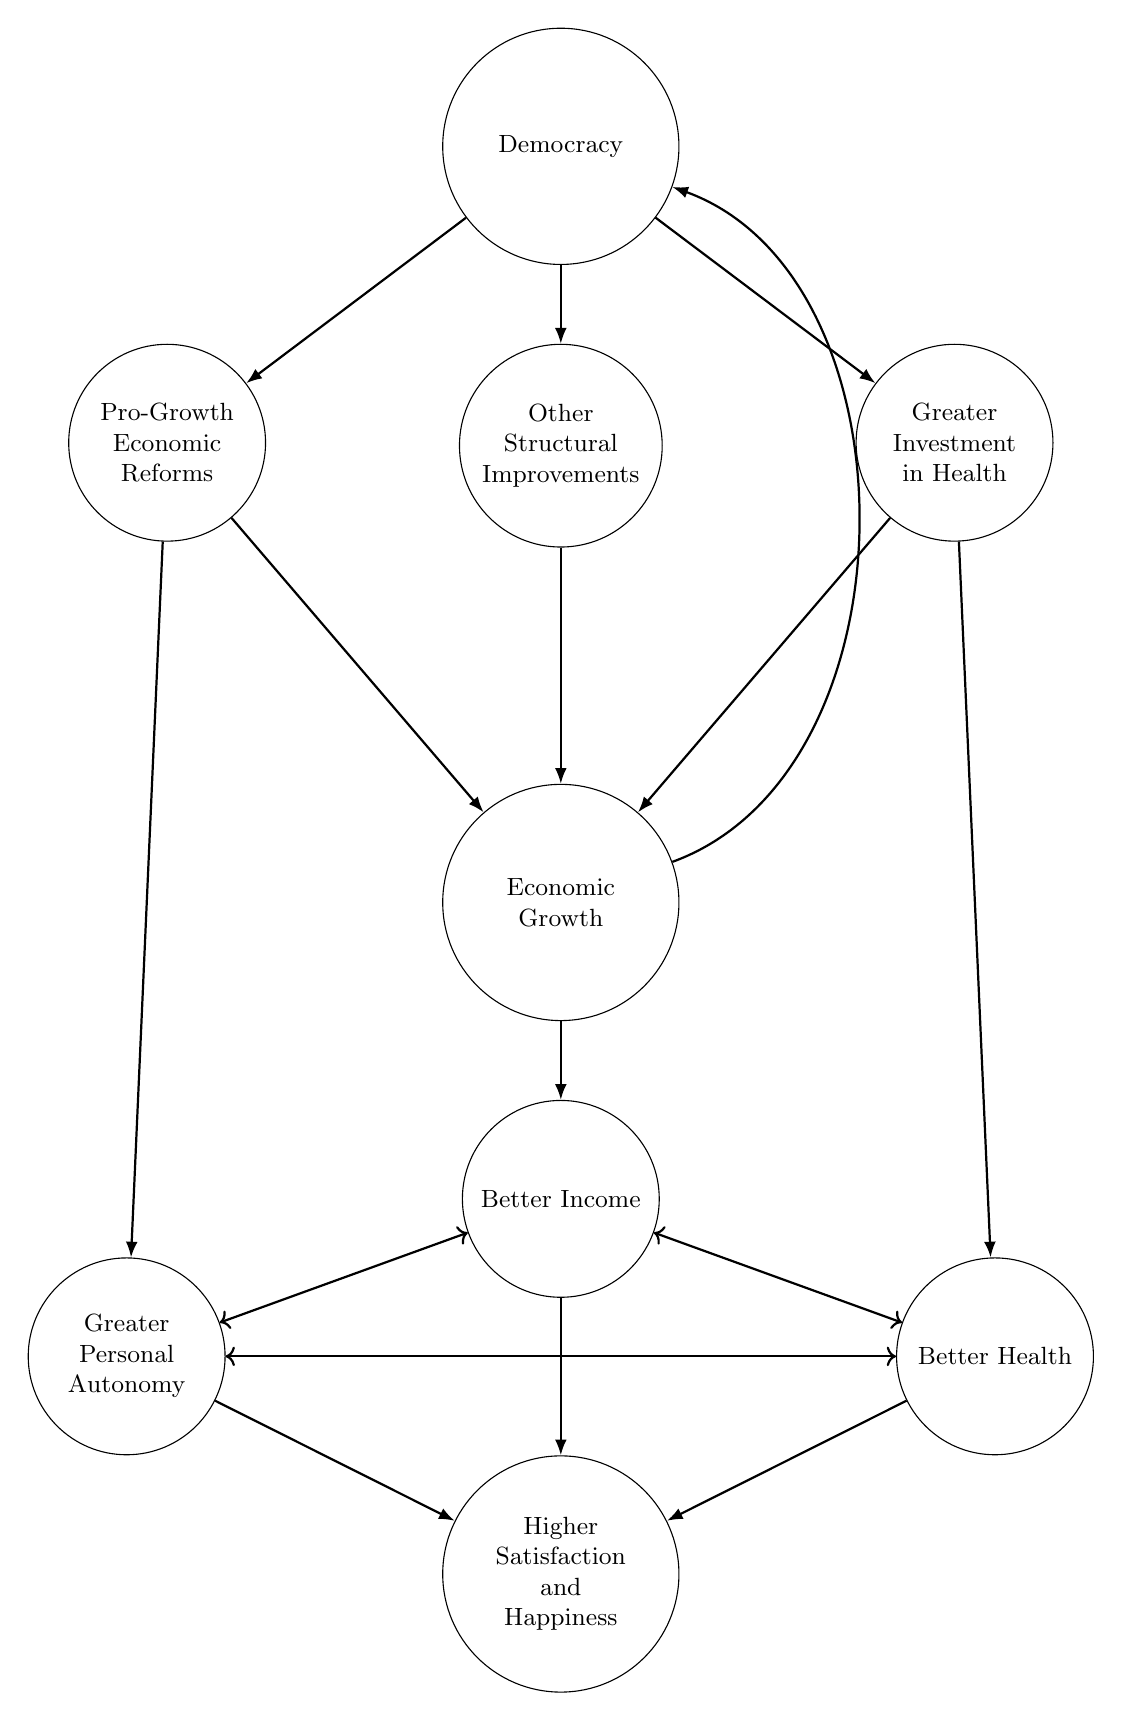
\begin{tikzpicture}[
		node distance=3cm and 2cm,
		node style/.style={draw, circle, minimum size=1.8cm, align=center, font=\small},
		arrow style/.style={-{Latex[length=2mm]}, thick}
		]
		
		% Nodo inicial
		\node[node style, minimum size=3cm] (democracy) {Democracy};
		
		% Nodos intermedios 
		\node[node style, below=1cm of democracy, xshift=-5cm, minimum size=2.5cm] (reform1) {Pro-Growth \\ Economic \\ Reforms};
		\node[node style, below=1cm of democracy, minimum size=2.5cm] (reform2) {Other \\ Structural \\ Improvements};
		\node[node style, below=1cm of democracy, xshift=5cm, minimum size=2.5cm] (reform3) {Greater \\ Investment \\ in Health};
		
		% Nodo de crecimiento
		\node[node style, below=3cm of reform2, minimum size=3cm] (growth) {Economic \\ Growth};
		
		% Nodos siguientes
		\node[node style, below=1cm of growth, xshift=0cm, minimum size=2.5cm] (income) {Better Income};
		\node[node style, right=3cm of income, xshift=0cm, yshift=-2cm, minimum size=2.5cm] (health) {Better Health};
		\node[node style, left=3cm of income, xshift=0cm, yshift=-2cm, minimum size=2.5cm] (autonomy) {Greater \\ Personal \\ Autonomy};
		
		% Nodos finales
		\node[node style, below=2cm of income, minimum size=3cm] (satisfaction) {Higher \\ Satisfaction \\ and \\ Happiness};
		
		% Flechas
		\draw[arrow style] (democracy) -- (reform1);
		\draw[arrow style] (democracy) -- (reform2);
		\draw[arrow style] (democracy) -- (reform3);
		
		\draw[arrow style] (reform1) -- (growth);
		\draw[arrow style] (reform1) -- (autonomy);
		\draw[arrow style] (reform2) -- (growth);
		\draw[arrow style] (reform3) -- (growth);
		\draw[arrow style] (reform3) -- (health);
		
		\draw[arrow style, bend left=290] (growth) to (democracy);
		
		\draw[arrow style] (growth) -- (income);
		\draw[arrow style, <->] (health) -- (autonomy);
		\draw[arrow style, <->] (income) -- (autonomy);
		\draw[arrow style, <->] (income) -- (health);
		\draw[arrow style] (health) -- (satisfaction);
		\draw[arrow style] (income) -- (satisfaction);
		\draw[arrow style] (autonomy) -- (satisfaction);
		
	\end{tikzpicture}
\end{figure}

\vspace*{2.5cm}
\begin{figure}[h]
	\begin{center}
		\caption{Pre-Birth Exposure to Democracy and Democracy 18-25}
		\label{figure2}
		
\includegraphics[scale=1]{\savef/befc1iy} 
	\end{center}
\end{figure}
\begin{center}
	\vspace{-1cm}
	\parbox{18cm}{\scriptsize \textbf{Notes:} Standard errors, robust to heteroskedasticity and serial correlation, are clustered at the country and survey-year levels and reported in parentheses. Results are shown separately for continuous and dichotomous measures of democracy. This figure plots OLS coefficient estimates for each one of our measures of well-being. This simultaneously includes Lifetime Exposure to Democracy and Pre-birth Exposure to Democracy. Pre-Birth Exposure to Democracy is constructed using a country’s democracy score before the relevant cohort’s birth. We take 10 years of placebo exposure in this case. For each outcome, in each panel, we show the placebo estimate (Pre-Birth Exposure to Democracy) from both specification 1 (red circles), and specification 2 (blue triangles). All regressions include fixed effects for: subregion, gender, language, wave of the survey, cohort, age and dummies of categories identifying the size of the city. The first specification adds fixed effects for country, year of interview and cohort. The second specification adds fixed effects for: region $\times$ year of interview and country $\times$ wave. We also report the estimates for Exposure to Democracy from the same specifications (our main variable of interest) for comparison. When the estimates for Exposure to Democracy are statistically different from the estimates for Pre-Birth Exposure to Democracy at 5\%, we depict them in black solid circles and triangles; when they are not statistically different, we depict them in grey hollowed circles and triangles. The whiskers indicate the 95 percent confidence intervals. All coefficients are standardized (beta coefficients). This figure uses V-DEM (1911-2023) and IVS (1981-2022) datasets.}
\end{center}

\vspace*{4cm}
\begin{figure}[h!]
	\begin{center}
		\caption{Placebo Variables 18-25}
		\label{figure3}
		%%%%%%%%%%%
		
\includegraphics[scale=1.1]{\savef/plaiy} 
	\end{center}
\end{figure}
\begin{center}
	\vspace{-1cm}
	\parbox{18cm}{\scriptsize \textbf{Notes:} Standard errors, robust to heteroskedasticity and serial correlation, are clustered at the country and survey-year levels and reported in parentheses. Results are shown separately for continuous and dichotomous measures of democracy. This figure plots OLS coefficient estimates of Lifetime Exposure to Democracy for various non-labor attitudinal questions. The left-hand side panel uses the dichotomous democracy score, while the right-hand side panel uses the continuous measure. All regressions include fixed effects following our baseline specification: gender, survey wave, birth cohort, age, language, town size, sub-region, country, and year of interview. The whiskers indicate the 95 percent confidence intervals. All coefficients are standardized (beta coefficients).}
\end{center}

\clearpage
\printbibliography

\clearpage
\section{Appendix}\label{sec:Appendix}
\setcounter{figure}{0}
\renewcommand{\thefigure}{A\arabic{figure}}
\setcounter{table}{0}
\renewcommand{\thetable}{A\arabic{table}}

\vspace*{-0.1cm}
\begin{table}[h!]
	\caption{Summary Statistics (1)}
	\label{at1}
	\par
	\begin{center}
		\scalebox{0.75}{
			\begin{tabular} {lcccccccc}
				\hline \hline
				&\multicolumn{6}{c}{\textit{Descriptive Statistics}} \\ 
				\cline{2-7}
				& \textbf{Observations} & \textbf{Mean} & \textbf{Median} & \textbf{SD} & \textbf{Min} & \textbf{Max} \\ 
				\hline \\
				\textit{A. Exposure.} \\
				\ExpandableInput{\savet/statsexposure}
				\hline \\
				\textit{B. Outcomes.} \\
				\ExpandableInput{\savet/statsoutcomes}
				\hline \\
				\textit{C. Pre-Birth.} \\
				\ExpandableInput{\savet/statsprebirth}
				\hline \\
				\textit{D. Placebo.} \\
				\ExpandableInput{\savet/statsplacebo}
				\hline \\
				\multicolumn{7}{l}{\parbox{18cm}{\footnotesize \textbf{Notes:} Countries in our IVS sample: 103, waves of survey: 12. This table uses IVS (1981-2022) and V-DEM (1911-2023).
				}}
			\end{tabular}
		}
	\end{center}
\end{table}

\clearpage
\begin{table}[h!]
	\caption{Summary Statistics (2)}
	\label{at2}
	\par
	\begin{center}
		\scalebox{0.75}{
			\begin{tabular} {lcccccccc}
				\hline \hline
				&\multicolumn{6}{c}{\textit{Descriptive Statistics}} \\ 
				\cline{2-7}
				& \textbf{Observations} & \textbf{Mean} & \textbf{Median} & \textbf{SD} & \textbf{Min} & \textbf{Max} \\ 
				\hline \\
				\textit{E. Mechanisms.} \\
				\ExpandableInput{\savet/statsmechanisms}
				\hline \\
				\textit{F. Fixed Effects, Clusters and Groups.} \\
				\ExpandableInput{\savet/statsfeclgr}
				\hline \\
				\textit{G. Alternative Outcomes} \\
				\ExpandableInput{\savet/statsapp}
				\ExpandableInput{\savet/statsess}
				\hline \\
				\multicolumn{7}{l}{\parbox{18cm}{\footnotesize \textbf{Notes:} Countries in our IVS sample: 103, waves of survey: 12. This table uses IVS (1981-2022) and V-DEM (1911-2023).
				}}
			\end{tabular}
		}
	\end{center}
\end{table}

\vspace*{0cm}
\begin{table}[h!]
	\caption{Survey Respondents by Region}
	\label{at3}
	\par
	\begin{center}
		\scalebox{0.8}{
			\begin{tabular}{lccc}
				\hline \hline
				\textbf{Region} & \textbf{Freq.} & \textbf{Percent} & \textbf{Cum.} \\
				\ExpandableInput{\savet/regions}
				\hline \\
				\multicolumn{4}{l}{\parbox{7.5cm}{\footnotesize \textbf{Notes:} Countries in our IVS sample: 103, waves of survey: 12.}}
			\end{tabular}	
		}
	\end{center}
\end{table}

\vspace*{0cm}
\begin{table}[h!]
	\caption{Exposure to Democracy 18-25 --- Diverse Fixed Effects}
	\label{at4}
	\begin{center}
		\scalebox{0.7}{
			\begin{tabular}{lcccccccccc}\hline \hline
				\ExpandableInput{\savet/headerFE.tex} 
				\hline \\
				\textbf{Income} \\ 
				\ExpandableInput{\savet/ftable_incomeiy.txt} \hline \\
				\textbf{Health} \\ 
				\ExpandableInput{\savet/ftable_healthiy.txt} \hline \\
				\textbf{Autonomy} \\ 
				\ExpandableInput{\savet/ftable_autonomyiy.txt} \hline \\
				\textbf{Satisfaction} \\ 
				\ExpandableInput{\savet/ftable_satisfactioniy.txt} \hline \\
				\textbf{Happiness} \\ 
				\ExpandableInput{\savet/ftable_happinessiy.txt} \hline \\
				\multicolumn{11}{l}{\parbox{23.5cm}{\footnotesize \textbf{Notes:}
						Standard errors, robust to heteroskedasticity and serial correlation, are clustered at the country and survey-year levels and reported in parentheses. Results are shown for the continuous measure of democracy. This table uses V-DEM (1911-2023) and IVS (1981-2022) datasets.
				}}
			\end{tabular}
		}
	\end{center}
\end{table}

\vspace*{0cm}
\begin{table}[h!]
	\caption{Exposure to Democracy 18-25 --- Diverse Clusters}
	\label{at5}
	\begin{center}
		\scalebox{0.7}{
			\begin{tabular}{lcccccccccc}\hline \hline
				\ExpandableInput{\savet/headerFE.tex} 
				\hline \\
				\textbf{Income} \\ 
				\ExpandableInput{\savet/ctable_incomeiy.txt} \hline \\
				\textbf{Health} \\ 
				\ExpandableInput{\savet/ctable_healthiy.txt} \hline \\
				\textbf{Autonomy} \\ 
				\ExpandableInput{\savet/ctable_autonomyiy.txt} \hline \\
				\textbf{Satisfaction} \\ 
				\ExpandableInput{\savet/ctable_satisfactioniy.txt} \hline \\
				\textbf{Happiness} \\ 
				\ExpandableInput{\savet/ctable_happinessiy.txt} \hline \\
				\multicolumn{11}{l}{\parbox{23.5cm}{\footnotesize \textbf{Notes:}
						Results are shown for the continuous measure of democracy. All regressions include fixed effects following our baseline specification: gender, survey wave, birth cohort, age, language, town size, sub-region, country, and year of interview. This table uses V-DEM (1911-2023) and IVS (1981-2022) datasets.
				}}
			\end{tabular}
		}
	\end{center}
\end{table}

\begin{table}[tbp]
	\caption{Lifetime Exposure to Democracy --- Capping Exposure to Democracy at 40}
	\label{at6}
	\begin{center}
		\scalebox{0.7}{
			\begin{tabular}{lccccc}
				\hline \hline
				\ExpandableInput{\savet/header}
				\\ 
				\textbf{Continuous} \\
				\ExpandableInput{\savet/demcapx2} \hline
				\\
				\textbf{Dichotomous} \\
				\ExpandableInput{\savet/demcapx1} \hline \\
				\multicolumn{6}{l}{\parbox{14.5cm}{\footnotesize \textbf{Notes:} 
						Standard errors, robust to heteroskedasticity and serial correlation, are clustered at the country and survey-year levels and reported in parentheses. Results are shown separately for continuous and dichotomous measures of democracy. Exposure to Democracy is capped at 40. All regressions include fixed effects following our baseline specification: gender, survey wave, birth cohort, age, language, town size, sub-region, country, and year of interview. All coefficients are standardized (beta coefficients). 
				}} \\
			\end{tabular}
		}
	\end{center}
\end{table}

\vspace*{0cm}
\begin{table}[h!]
	\caption{Exposure to Democracy 18–25 --- Leave-One-Out and Europe-Only}
	\label{at7}
	\begin{center}
		\scalebox{0.7}{
			\begin{tabular}{lccccc}\hline \hline
				\ExpandableInput{\savet/header.tex} 
				\hline \\
				\textbf{Without Africa} \\
				\ExpandableInput{\savet/x2s1c1iy_noAfrica} \hline \\
				\textbf{Without Asia} \\
				\ExpandableInput{\savet/x2s1c1iy_noAsia} \hline \\
				\textbf{Without Europe} \\
				\ExpandableInput{\savet/x2s1c1iy_noEurope} \hline \\
				\textbf{Without Latin America} \\
				\ExpandableInput{\savet/x2s1c1iy_noLatin_America} \hline \\
				\textbf{Without Anglo-Saxon America} \\
				\ExpandableInput{\savet/x2s1c1iy_noAS_America} \hline \\
				\textbf{Without Oceania} \\
				\ExpandableInput{\savet/x2s1c1iy_noOceania} \hline \\ 
				\textbf{Only Europe} \\
				\ExpandableInput{\savet/x2s1c1iy_Europe} \hline \\
				\multicolumn{6}{l}{\parbox{16.5cm}{\footnotesize \textbf{Notes:}
						Standard errors, robust to heteroskedasticity and serial correlation, are clustered at the country and survey-year levels and reported in parentheses. Results are shown for the continuous measure of democracy. *** Significant at the 1\% level; ** Significant at the 5\% level; * Significant at the 10\% level. All continuous outcomes and independent variables are normalized by their standard deviations. Each of these variables includes an additional category for missing values. All regressions include fixed effects following our baseline specification: gender, survey wave, birth cohort, age, language, town size, sub-region, country, and year of interview. This table uses V-DEM (1911-2023) and IVS (1981-2022) datasets.
				}}
			\end{tabular}
		}
	\end{center}
\end{table}

\vspace*{0cm}
\begin{table}[h!]
	\caption{Lifetime Exposure to Democracy --- Leave-One-Out and Europe-Only}
	\label{at8}
	\begin{center}
		\scalebox{0.7}{
			\begin{tabular}{lccccc}\hline \hline
				\ExpandableInput{\savet/header.tex} 
				\hline \\
				\textbf{Without Africa} \\
				\ExpandableInput{\savet/x2s1c1lt_noAfrica} \hline \\
				\textbf{Without Asia} \\
				\ExpandableInput{\savet/x2s1c1lt_noAsia} \hline \\
				\textbf{Without Europe} \\
				\ExpandableInput{\savet/x2s1c1lt_noEurope} \hline \\
				\textbf{Without Latin America} \\
				\ExpandableInput{\savet/x2s1c1lt_noLatin_America} \hline \\
				\textbf{Without Anglo-Saxon America} \\
				\ExpandableInput{\savet/x2s1c1lt_noAS_America} \hline \\
				\textbf{Without Oceania} \\
				\ExpandableInput{\savet/x2s1c1lt_noOceania} \hline \\ 
				\textbf{Only Europe} \\
				\ExpandableInput{\savet/x2s1c1lt_Europe} \hline \\
				\multicolumn{6}{l}{\parbox{16.5cm}{\footnotesize \textbf{Notes:}
						Standard errors, robust to heteroskedasticity and serial correlation, are clustered at the country and survey-year levels and reported in parentheses. Results are shown for the continuous measure of democracy. *** Significant at the 1\% level; ** Significant at the 5\% level; * Significant at the 10\% level. All continuous outcomes and independent variables are normalized by their standard deviations. Each of these variables includes an additional category for missing values. All regressions include fixed effects following our baseline specification: gender, survey wave, birth cohort, age, language, town size, sub-region, country, and year of interview. This table uses V-DEM (1911-2023) and IVS (1981-2022) datasets.
				}}
			\end{tabular}
		}
	\end{center}
\end{table}

\vspace*{0cm}
\begin{table}[h!]
	\caption{Exposure to Democracy 18-25 --- Heterogeneities}
	\label{at9}
	\begin{center}
		\scalebox{0.68}{
			\begin{tabular}{lccccc}\hline \hline
				\ExpandableInput{\savet/header.tex} 
				\hline \\
				\textbf{Only Female} \\
				\ExpandableInput{\savet/x2s1c1iy_male0} \hline \\
				\textbf{Only Male} \\
				\ExpandableInput{\savet/x2s1c1iy_male1} \hline \\
				\textbf{Only Big Cities} \\
				\ExpandableInput{\savet/x2s1c1iy_town0} \hline \\
				\textbf{Only Small Cities} \\
				\ExpandableInput{\savet/x2s1c1iy_town1} \hline \\
				\textbf{Only Young} \\
				\ExpandableInput{\savet/x2s1c1iy_age1} \hline \\
				\textbf{Only Middle-aged} \\
				\ExpandableInput{\savet/x2s1c1iy_age2} \hline \\
				\textbf{Only Old People} \\
				\ExpandableInput{\savet/x2s1c1iy_age3} \hline \\
				\textbf{Only Left-Wing} \\
				\ExpandableInput{\savet/x2s1c1iy_pol1} \hline \\
				\textbf{Only Centrists} \\
				\ExpandableInput{\savet/x2s1c1iy_pol2} \hline \\
				\textbf{Only Right-Wing} \\
				\ExpandableInput{\savet/x2s1c1iy_pol3} \hline \\
				\multicolumn{6}{l}{\parbox{16cm}{\footnotesize \textbf{Notes:}
						Standard errors, robust to heteroskedasticity and serial correlation, are clustered at the country and survey-year levels and reported in parentheses. Results are shown for the continuous measure of democracy. *** Significant at the 1\% level; ** Significant at the 5\% level; * Significant at the 10\% level. All continuous outcomes and independent variables are normalized by their standard deviations. Each of these variables includes an additional category for missing values. All regressions include fixed effects following our baseline specification: gender, survey wave, birth cohort, age, language, town size, sub-region, country, and year of interview. This table uses V-DEM (1911-2023) and IVS (1981-2022) datasets.
				}}
			\end{tabular}
		}
	\end{center}
\end{table}

\vspace*{0cm}
\begin{table}[h!]
	\caption{Exposure to Democracy 18-25 --- Alternative Mechanisms, Religion and Beliefs}
	\label{at10}
	\begin{center}
		\scalebox{0.7}{
			\begin{tabular}{lccccccc}\hline \hline
				\ExpandableInput{\savet/i1.tex} 
				\hline \\
				\textbf{Continuous} \\
				\hline \\
				\ExpandableInput{\savet/i1x2s1c1iy} \hline \\
				\textbf{Dichotomous} \\
				\hline \\
				\ExpandableInput{\savet/i1x1s1c1iy} \hline \\
				\multicolumn{7}{l}{\parbox{22cm}{\footnotesize \textbf{Notes:}
						Standard errors, robust to heteroskedasticity and serial correlation, are clustered at the country and survey-year levels and reported in parentheses. Results are shown separately for continuous and dichotomous measures of democracy. *** Significant at the 1\% level; ** Significant at the 5\% level; * Significant at the 10\% level. All continuous outcomes and independent variables are normalized by their standard deviations. Each of these variables includes an additional category for missing values. All regressions include fixed effects following our baseline specification: gender, survey wave, birth cohort, age, language, town size, sub-region, country, and year of interview. This table uses V-DEM (1911-2023) and IVS (1981-2022) datasets.
				}}
			\end{tabular}
		}
	\end{center}
\end{table}

\vspace*{0cm}
\begin{table}[h!]
	\caption{Exposure to Democracy 18-25 --- Alternative Mechanisms, Education}
	\label{at11}
	\begin{center}
		\scalebox{0.7}{
			\begin{tabular}{lcccc}\hline \hline
				\ExpandableInput{\savet/i2.tex} 
				\hline \\
				\textbf{Continuous} \\
				\hline \\
				\ExpandableInput{\savet/i2x2s1c1iy} \hline \\
				\textbf{Dichotomous} \\
				\hline \\
				\ExpandableInput{\savet/i2x1s1c1iy} \hline \\
				\multicolumn{4}{l}{\parbox{16cm}{\footnotesize \textbf{Notes:}
						Standard errors, robust to heteroskedasticity and serial correlation, are clustered at the country and survey-year levels and reported in parentheses. Results are shown separately for continuous and dichotomous measures of democracy. *** Significant at the 1\% level; ** Significant at the 5\% level; * Significant at the 10\% level. All continuous outcomes and independent variables are normalized by their standard deviations. Each of these variables includes an additional category for missing values. All regressions include fixed effects following our baseline specification: gender, survey wave, birth cohort, age, language, town size, sub-region, country, and year of interview. This table uses V-DEM (1911-2023) and IVS (1981-2022) datasets.
				}}
			\end{tabular}
		}
	\end{center}
\end{table}

\vspace*{0cm}
\begin{table}[h!]
	\caption{Exposure to Democracy 18-25 --- Alternative Mechanisms, Employment}
	\label{at12}
	\begin{center}
		\scalebox{0.7}{
			\begin{tabular}{lccccccccccccc}\hline \hline
				\ExpandableInput{\savet/i3.tex} 
				\hline \\
				\textbf{Continuous} \\
				\hline \\
				\ExpandableInput{\savet/i3x2s1c1iy} \hline \\
				\textbf{Dichotomous} \\
				\hline \\
				\ExpandableInput{\savet/i3x1s1c1iy} \hline \\
				\multicolumn{8}{l}{\parbox{20.5cm}{\footnotesize \textbf{Notes:}
						Standard errors, robust to heteroskedasticity and serial correlation, are clustered at the country and survey-year levels and reported in parentheses. Results are shown separately for continuous and dichotomous measures of democracy. *** Significant at the 1\% level; ** Significant at the 5\% level; * Significant at the 10\% level. All continuous outcomes and independent variables are normalized by their standard deviations. Each of these variables includes an additional category for missing values. All regressions include fixed effects following our baseline specification: gender, survey wave, birth cohort, age, language, town size, sub-region, country, and year of interview. This table uses V-DEM (1911-2023) and IVS (1981-2022) datasets.
				}}
			\end{tabular}
		}
	\end{center}
\end{table}

\vspace*{0cm}
\begin{table}[h!]
	\caption{Exposure to Democracy 18-25 --- Alternative Mechanisms, Security and Fear}
	\label{at13}
	\begin{center}
		\scalebox{0.7}{
			\begin{tabular}{lccccccccccccc}\hline \hline
				\ExpandableInput{\savet/i4.tex} 
				\hline \\
				\textbf{Continuous} \\
				\hline \\
				\ExpandableInput{\savet/i4x2s1c1iy} \hline \\
				\textbf{Dichotomous} \\
				\hline \\
				\ExpandableInput{\savet/i4x1s1c1iy} \hline \\
				\multicolumn{8}{l}{\parbox{23cm}{\footnotesize \textbf{Notes:}
						Standard errors, robust to heteroskedasticity and serial correlation, are clustered at the country and survey-year levels and reported in parentheses. Results are shown separately for continuous and dichotomous measures of democracy. *** Significant at the 1\% level; ** Significant at the 5\% level; * Significant at the 10\% level. All continuous outcomes and independent variables are normalized by their standard deviations. Each of these variables includes an additional category for missing values. All regressions include fixed effects following our baseline specification: gender, survey wave, birth cohort, age, language, town size, sub-region, country, and year of interview. This table uses V-DEM (1911-2023) and IVS (1981-2022) datasets.
				}}
			\end{tabular}
		}
	\end{center}
\end{table}

\begin{table}[h!]
	\caption{2SLS Estimation 18-25 --- First-Stage Regression}
	\label{at14}
	\begin{center}
		\scalebox{0.7}{
			\begin{tabular}{lcc}\hline \hline
				\ExpandableInput{\savet/headerFSIY.tex} 
				\hline \\
				\textbf{Continuous} \\
				\hline \\
				\ExpandableInput{\savet//fsdemx2iy} \hline \\
				\textbf{Dichotomous} \\
				\hline \\
				\ExpandableInput{\savet//fsdemx1iy} \hline \\
				\multicolumn{3}{l}{\parbox{11cm}{\footnotesize \textbf{Notes:}
						Standard errors, robust to heteroskedasticity and serial correlation, are clustered at the country and survey-year levels and reported in parentheses. Results are shown separately for continuous and dichotomous measures of democracy. *** Significant at the 1\% level; ** Significant at the 5\% level; * Significant at the 10\% level. All continuous outcomes and independent variables are normalized by their standard deviations. Each of these variables includes an additional category for missing values. All regressions include fixed effects following our baseline specification: gender, survey wave, birth cohort, age, language, town size, sub-region, country, and year of interview. The first-stage F-statistic is reported below the coefficient estimates. The instrument for Exposure to Democracy is constructed using regional waves of democratization as Acemoglu et al. (2019). This table uses V-DEM (1911-2023) and IVS (1981-2022) datasets.
				}}
			\end{tabular}
		}
	\end{center}
\end{table}

\begin{table}[h!]
	\caption{IV Exposure to Democracy 18-25}
	\label{at15}
	\begin{center}
		\scalebox{0.7}{
			\begin{tabular}{lccccc}\hline \hline
				\ExpandableInput{\savet/header.tex} 
				\hline \\
				\textbf{Continuous} \\
				\hline \\
				\ExpandableInput{\savet//ivdemx2s1iy} \hline \\
				\textbf{Dichotomous} \\
				\hline \\
				\ExpandableInput{\savet//ivdemx1s1iy} \hline \\
				\multicolumn{6}{l}{\parbox{15.5cm}{\footnotesize \textbf{Notes:}
						Standard errors, robust to heteroskedasticity and serial correlation, are clustered at the country and survey-year levels and reported in parentheses. Results are shown separately for continuous and dichotomous measures of democracy. *** Significant at the 1\% level; ** Significant at the 5\% level; * Significant at the 10\% level. All continuous outcomes and independent variables are normalized by their standard deviations. Each of these variables includes an additional category for missing values. All regressions include fixed effects following our baseline specification: gender, survey wave, birth cohort, age, language, town size, sub-region, country, and year of interview. This table uses V-DEM (1911-2023) and IVS (1981-2022) datasets.
				}}
			\end{tabular}
		}
	\end{center}
\end{table}

\begin{table}[h!]
	\caption{2SLS Estimation Lifetime --- First-Stage Regression}
	\label{at16}
	\begin{center}
		\scalebox{0.7}{
			\begin{tabular}{lcc}\hline \hline
				\ExpandableInput{\savet/headerFS.tex} 
				\hline \\
				\textbf{Continuous} \\
				\hline \\
				\ExpandableInput{\savet//fsdemx2lt} \hline \\
				\textbf{Dichotomous} \\
				\hline \\
				\ExpandableInput{\savet//fsdemx1lt} \hline \\
				\multicolumn{3}{l}{\parbox{10cm}{\footnotesize \textbf{Notes:}
						Standard errors, robust to heteroskedasticity and serial correlation, are clustered at the country and survey-year levels and reported in parentheses. Results are shown separately for continuous and dichotomous measures of democracy. *** Significant at the 1\% level; ** Significant at the 5\% level; * Significant at the 10\% level. All continuous outcomes and independent variables are normalized by their standard deviations. Each of these variables includes an additional category for missing values. All regressions include fixed effects following our baseline specification: gender, survey wave, birth cohort, age, language, town size, sub-region, country, and year of interview. The first-stage F-statistic is reported below the coefficient estimates. The instrument for Exposure to Democracy is constructed using regional waves of democratization as Acemoglu et al. (2019). This table uses V-DEM (1911-2023) and IVS (1981-2022) datasets.
				}}
			\end{tabular}
		}
	\end{center}
\end{table}

\begin{table}[h!]
	\caption{IV Lifetime Exposure to Democracy}
	\label{at17}
	\begin{center}
		\scalebox{0.7}{
			\begin{tabular}{lccccc}\hline \hline
				\ExpandableInput{\savet/header.tex} 
				\hline \\
				\textbf{Continuous} \\
				\hline \\
				\ExpandableInput{\savet//ivdemx2s1lt} \hline \\
				\textbf{Dichotomous} \\
				\hline \\
				\ExpandableInput{\savet//ivdemx1s1lt} \hline \\
				\multicolumn{6}{l}{\parbox{14.5cm}{\footnotesize \textbf{Notes:}
						Standard errors, robust to heteroskedasticity and serial correlation, are clustered at the country and survey-year levels and reported in parentheses. Results are shown separately for continuous and dichotomous measures of democracy. *** Significant at the 1\% level; ** Significant at the 5\% level; * Significant at the 10\% level. All continuous outcomes and independent variables are normalized by their standard deviations. Each of these variables includes an additional category for missing values. All regressions include fixed effects following our baseline specification: gender, survey wave, birth cohort, age, language, town size, sub-region, country, and year of interview. This table uses V-DEM (1911-2023) and IVS (1981-2022) datasets.
				}}
			\end{tabular}
		}
	\end{center}
\end{table}

\begin{table}[tbp]
	\caption{Exposure to Democracy --- Event-specific Estimates}
	\label{at18}
	\begin{center}
		\scalebox{0.7}{
			\begin{tabular}{lccccc}
				\hline \hline
				\ExpandableInput{\savet/header}
				 \hline \\
				\multicolumn{1}{l}{\textbf{HTEE}} \\
				\ExpandableInput{\savet/eventdemx1s1} \hline \\
				\multicolumn{1}{l}{\textbf{HTEE and Length of the Exposure}} \\
				\ExpandableInput{\savet/eventdemx1s1Years5} \hline \\
				\multicolumn{6}{l}{\parbox{17.5cm}{\footnotesize \textbf{Notes:} 
						This table reports event-specific estimates of Lifetime Exposure to Democracy on our outcomes robust to heterogeneous treatment effects, based on  \bbb{Wooldridge2021}. The first panel reports the inverse-variance-weighted average of event-specific estimates resulting from an extended version of equation \eqref{2} that allows the effect of Lifetime Exposure to Democracy to be heterogenous by event (a unique spell of democracy in a country). The HTEE means Heterogeneous Treatment Effects by Event. The second panel extends this estimate to allow for treatment heterogeneity both across events and time of the exposure (five-year periods in the duration of the event for each individual). So, the last panel accounts for HTEE and Length of the Exposure in 5-year periods. All regressions are based on the dichotomous democratic score and include a full set of fixed effects following our baseline specification: gender, survey wave, birth cohort, age, language, town size, sub-region, country, and year of interview. All coefficients are standardized (beta coefficients). Standard errors, robust to heteroskedasticity and serial correlation, are clustered at the country and survey-year levels and reported in parentheses. The standard errors for the inverse-variance-weighted average are computed based on the delta method.
				}} \\
				
			\end{tabular}
		}
	\end{center}
\end{table}

\vspace*{3cm}
\begin{table}[h!]
	\caption{Exposure to Democracy and Well-Being --- ESS Sample}
	\label{at19}
	\begin{center}
		\scalebox{0.75}{
			\begin{tabular}{lccccc}\hline \hline
				\ExpandableInput{\savet/header.tex} 
				\hline \\
				\multicolumn{1}{l}{\textbf{Continuous Democracy 18-25}} \\
				\\
				\ExpandableInput{\savet/x2s1c1iyess} \hline \\
				\multicolumn{6}{l}{\textbf{Dichotomous Democracy 18-25}} \\
				\\
				\ExpandableInput{\savet/x1s1c1iyess} \hline \\
				\multicolumn{6}{l}{\textbf{Continuous Lifetime Democracy}} \\
				\\
				\ExpandableInput{\savet/x2s1c1ltess} \hline \\
				\multicolumn{1}{l}{\textbf{Dichotomous Lifetime Democracy}} \\
				\\
				\ExpandableInput{\savet/x1s1c1ltess} \hline \\
				\multicolumn{6}{l}{\parbox{17cm}{\footnotesize \textbf{Notes:}
						Standard errors, robust to heteroskedasticity and serial correlation, are clustered at the country and survey-year levels and reported in parentheses. Results are shown separately for continuous and dichotomous measures of democracy. *** Significant at the 1\% level; ** Significant at the 5\% level; * Significant at the 10\% level. All continuous outcomes and independent variables are normalized by their standard deviations. Each of these variables includes an additional category for missing values. All regressions include fixed effects for: gender, survey wave, birth cohort, age, country, and year of interview. This table uses V-DEM (1911-2023) and ESS (2002-2018) datasets.
				}}
			\end{tabular}
		}
	\end{center}
\end{table}

\vspace*{3cm}
\begin{table}[h!]
	\caption{Exposure to Democracy and Well-Being --- Immigrants}
	\label{at20}
	\begin{center}
		\scalebox{0.75}{
			\begin{tabular}{lccccc}\hline \hline
				\ExpandableInput{\savet/header.tex} 
				\hline \\
				\multicolumn{1}{l}{\textbf{Continuous Democracy 18-25, Specification 1}} \\
				\\
				\ExpandableInput{\savet/x2s1c1iyessi1} \hline \\
				\multicolumn{1}{l}{\textbf{Continuous Democracy 18-25, Specification 2}} \\
				\\
				\ExpandableInput{\savet/x2s1c1iyessi2} \hline \\
				\multicolumn{1}{l}{\textbf{Continuous Democracy 18-25, Specification 3}} \\
				\\
				\ExpandableInput{\savet/x2s1c1iyessi3} \hline \\
				\multicolumn{1}{l}{\textbf{Dichotomous Democracy 18-25, Specification 1}} \\
				\\
				\ExpandableInput{\savet/x1s1c1iyessi1} \hline \\
				\multicolumn{1}{l}{\textbf{Dichotomous Democracy 18-25, Specification 2}} \\
				\\
				\ExpandableInput{\savet/x1s1c1iyessi2} \hline \\
				\multicolumn{1}{l}{\textbf{Dichotomous Democracy 18-25, Specification 3}} \\
				\\
				\ExpandableInput{\savet/x1s1c1iyessi3} \hline \\
				\multicolumn{6}{l}{\parbox{19.5cm}{\footnotesize \textbf{Notes:}
						Standard errors, robust to heteroskedasticity and serial correlation, are clustered at the country and survey-year levels and reported in parentheses. Results are shown separately for continuous and dichotomous measures of democracy. *** Significant at the 1\% level; ** Significant at the 5\% level; * Significant at the 10\% level. All continuous outcomes and independent variables are normalized by their standard deviations. Each of these variables includes an additional category for missing values. Specification 1 uses survey-year, migration-year, birth-cohort, age, gender, and wave fixed effects to absorb broad temporal and demographic heterogeneity. Specification 2 replaces these with country-by-birth-year fixed effects, tightening identification by comparing individuals from the same origin-cohort. Specification 3 incorporates joint birth-year-by-migration-year fixed effects, ensuring that identification comes solely from the timing of institutional exposure in the origin country while controlling for age, gender, and survey-year. This table uses V-DEM (1911-2023) and ESS (2002-2018) datasets.
				}}
			\end{tabular}
		}
	\end{center}
\end{table}

\clearpage
\vspace*{0.7cm}
\begin{figure}[h!]
	\caption{Democracy and Exposure to Democracy by Year/Cohort}
	\label{af1}
	\vspace{-0.5cm}
\end{figure}
%%%%%%%%%%%
\begin{center}
	\scalebox{1}{
		\begin{tabular}{cc}
			{A. Yearly values of Continuous Democracy, from 1918 to 2023}\\
			
\includegraphics[scale=0.8]{\savef/dem2_selected_countries} \\
			{B. Exposure to Democracy 18-25 by cohort, from 1900 to 2000} \\
			
\includegraphics[scale=0.8]{\savef/exp_dem2_selected_countries} \\
		\end{tabular}
	} 
	\parbox{14cm}{\scriptsize \textbf{Notes:} The Democracy Index is the average of the five V-Dem components of democracy (electoral, liberal, participatory, deliberative, and egalitarian) and ranges from 0 to 1. Democracy 18–25 is defined as the average democracy score a cohort experiences between ages 18 and 25. It is calculated as the mean of the yearly Democracy Index values over this fixed eight-year window. Because the window length is constant, this average is equivalent to a rescaled version of the cumulative exposure measure used in the regressions. The figure displays all countries included in the Integrated Values Surveys and is based on the V-Dem dataset (1911–2023).}
\end{center}

\vspace*{3cm}
\begin{figure}[h]
	\begin{center}
		\caption{Pre-Birth Exposure to Democracy and Lifetime Democracy}
		\label{af2}
		
\includegraphics[scale=1]{\savef/befc1lt} 
	\end{center}
\end{figure}
\begin{center}
	\vspace{-1cm}
	\parbox{18cm}{\scriptsize \textbf{Notes:} Standard errors, robust to heteroskedasticity and serial correlation, are clustered at the country and survey-year levels and reported in parentheses. Results are shown separately for continuous and dichotomous measures of democracy. This figure plots OLS coefficient estimates for each one of our measures of well-being. This simultaneously includes Lifetime Exposure to Democracy and Pre-birth Exposure to Democracy. Pre-Birth Exposure to Democracy is constructed using a country’s democracy score before the relevant cohort’s birth. We take 10 years of placebo exposure in this case. For each outcome, in each panel, we show the placebo estimate (Pre-Birth Exposure to Democracy) from both specification 1 (red circles), and specification 2 (blue triangles). All regressions include fixed effects for: subregion, gender, language, wave of the survey, cohort, age and dummies of categories identifying the size of the city. The first specification adds fixed effects for country, year of interview and cohort. The second specification adds fixed effects for: region $\times$ year of interview and country $\times$ wave. We also report the estimates for Exposure to Democracy from the same specifications (our main variable of interest) for comparison. When the estimates for Exposure to Democracy are statistically different from the estimates for Pre-Birth Exposure to Democracy at 5\%, we depict them in black solid circles and triangles; when they are not statistically different, we depict them in grey hollowed circles and triangles. The whiskers indicate the 95 percent confidence intervals. All coefficients are standardized (beta coefficients). This figure uses V-DEM (1911-2023) and IVS (1981-2022) datasets.}
\end{center}


\vspace*{4cm}
\begin{figure}[h]
	\begin{center}
		\caption{Pre-Birth Exposure to Successful Democracy and Successful Democracy 18-25}
		\label{af3}
		
\includegraphics[scale=0.9]{\savef/befsuc1iy} 
	\end{center}
\end{figure}
\begin{center}
	\vspace{-1cm}
	\parbox{18cm}{\scriptsize \textbf{Notes:} Standard errors, robust to heteroskedasticity and serial correlation, are clustered at the country and survey-year levels and reported in parentheses. Results are shown separately for continuous and dichotomous measures of democracy. This figure plots OLS coefficient estimates for each one of our measures of well-being. This simultaneously includes Exposure to Successful Democracy 18-25 and Pre-birth Exposure to Democracy. Pre-Birth Exposure to Democracy is constructed using a country’s democracy score before the relevant cohort’s birth. We take 10 years of placebo exposure in this case. For each outcome, in each panel, we show the placebo estimate (Pre-Birth Exposure to Democracy) from both specification 1 (red circles), and specification 2 (blue triangles). All regressions include fixed effects for: subregion, gender, language, wave of the survey, cohort, age and dummies of categories identifying the size of the city. The first specification adds fixed effects for country, year of interview and cohort. The second specification adds fixed effects for: region $\times$ year of interview and country $\times$ wave. We also report the estimates for Exposure to Democracy from the same specifications (our main variable of interest) for comparison. When the estimates for Exposure to Democracy are statistically different from the estimates for Pre-Birth Exposure to Democracy at 5\%, we depict them in black solid circles and triangles; when they are not statistically different, we depict them in grey hollowed circles and triangles. The whiskers indicate the 95 percent confidence intervals. All coefficients are standardized (beta coefficients). This figure uses V-DEM (1911-2023) and IVS (1981-2022) datasets.}
\end{center}

\vspace*{4cm}
\begin{figure}[h]
	\begin{center}
		\caption{Pre-Birth Exposure to Unsuccessful Democracy and Unsuccessful Autocracy, 18-25}
		\label{af4}
		
\includegraphics[scale=0.9]{\savef/befsuc2iy} 
	\end{center}
\end{figure}
\begin{center}
	\vspace{-1cm}
	\parbox{18cm}{\scriptsize \textbf{Notes:} Standard errors, robust to heteroskedasticity and serial correlation, are clustered at the country and survey-year levels and reported in parentheses. Results are shown separately for continuous and dichotomous measures of democracy. This figure plots OLS coefficient estimates for each one of our measures of well-being. This simultaneously includes Exposure to Unsuccessful Democracy and Pre-birth Exposure to Democracy, or Exposure to Unsuccessful Autocracy and Pre-birth Exposure to Democracy. Pre-Birth Exposure to Democracy is constructed using a country’s democracy score before the relevant cohort’s birth. We take 10 years of placebo exposure in this case. For each outcome, in each panel, we show the placebo estimate (Pre-Birth Exposure to Democracy) from both specification 1 (red circles), and specification 2 (blue triangles). All regressions include fixed effects for: subregion, gender, language, wave of the survey, cohort, age and dummies of categories identifying the size of the city. The first specification adds fixed effects for country, year of interview and cohort. The second specification adds fixed effects for: region $\times$ year of interview and country $\times$ wave. We also report the estimates for Exposure to Democracy from the same specifications (our main variable of interest) for comparison. When the estimates for Exposure to Democracy are statistically different from the estimates for Pre-Birth Exposure to Democracy at 5\%, we depict them in black solid circles and triangles; when they are not statistically different, we depict them in grey hollowed circles and triangles. The whiskers indicate the 95 percent confidence intervals. All coefficients are standardized (beta coefficients). This figure uses V-DEM (1911-2023) and IVS (1981-2022) datasets.}
\end{center}

\vspace*{4cm}
\begin{figure}[h]
	\begin{center}
		\caption{Pre-Birth Exposure to Successful Democracy and Lifetime Successful Democracy}
		\label{af5}
		
\includegraphics[scale=0.9]{\savef/befsuc1lt} 
	\end{center}
\end{figure}
\begin{center}
	\vspace{-1cm}
	\parbox{18cm}{\scriptsize \textbf{Notes:} Standard errors, robust to heteroskedasticity and serial correlation, are clustered at the country and survey-year levels and reported in parentheses. Results are shown separately for continuous and dichotomous measures of democracy. This figure plots OLS coefficient estimates for each one of our measures of well-being. This simultaneously includes Lifetime Exposure to Democracy and Pre-birth Exposure to Democracy. Pre-Birth Exposure to Democracy is constructed using a country’s democracy score before the relevant cohort’s birth. We take 10 years of placebo exposure in this case. For each outcome, in each panel, we show the placebo estimate (Pre-Birth Exposure to Democracy) from both specification 1 (red circles), and specification 2 (blue triangles). All regressions include fixed effects for: subregion, gender, language, wave of the survey, cohort, age and dummies of categories identifying the size of the city. The first specification adds fixed effects for country, year of interview and cohort. The second specification adds fixed effects for: region $\times$ year of interview and country $\times$ wave. We also report the estimates for Exposure to Democracy from the same specifications (our main variable of interest) for comparison. When the estimates for Exposure to Democracy are statistically different from the estimates for Pre-Birth Exposure to Democracy at 5\%, we depict them in black solid circles and triangles; when they are not statistically different, we depict them in grey hollowed circles and triangles. The whiskers indicate the 95 percent confidence intervals. All coefficients are standardized (beta coefficients). This figure uses V-DEM (1911-2023) and IVS (1981-2022) datasets.}
\end{center}

\vspace*{4cm}
\begin{figure}[h]
	\begin{center}
		\caption{Pre-Birth Exposure to Unsuccessful Democracy and Unsuccessful Autocracy, Lifetime}
		\label{af6}
		
\includegraphics[scale=0.9]{\savef/befsuc2lt} 
	\end{center}
\end{figure}
\begin{center}
	\vspace{-1cm}
	\parbox{18cm}{\scriptsize \textbf{Notes:} Standard errors, robust to heteroskedasticity and serial correlation, are clustered at the country and survey-year levels and reported in parentheses. Results are shown separately for continuous and dichotomous measures of democracy. This figure plots OLS coefficient estimates for each one of our measures of well-being. This simultaneously includes Lifetime Exposure to Democracy and Pre-birth Exposure to Democracy. Pre-Birth Exposure to Democracy is constructed using a country’s democracy score before the relevant cohort’s birth. We take 10 years of placebo exposure in this case. For each outcome, in each panel, we show the placebo estimate (Pre-Birth Exposure to Democracy) from both specification 1 (red circles), and specification 2 (blue triangles). All regressions include fixed effects for: subregion, gender, language, wave of the survey, cohort, age and dummies of categories identifying the size of the city. The first specification adds fixed effects for country, year of interview and cohort. The second specification adds fixed effects for: region $\times$ year of interview and country $\times$ wave. We also report the estimates for Exposure to Democracy from the same specifications (our main variable of interest) for comparison. When the estimates for Exposure to Democracy are statistically different from the estimates for Pre-Birth Exposure to Democracy at 5\%, we depict them in black solid circles and triangles; when they are not statistically different, we depict them in grey hollowed circles and triangles. The whiskers indicate the 95 percent confidence intervals. All coefficients are standardized (beta coefficients). This figure uses V-DEM (1911-2023) and IVS (1981-2022) datasets.}
\end{center}

\clearpage
\begin{figure}[h!]
	\begin{center}
		\caption{Success in Europe and Asia}
		\label{af7}
		
\includegraphics[scale=0.8]{\savef/europevsasia} 
	\end{center}
\end{figure}
\begin{center}
	\vspace{-1.5cm}
	\parbox{18cm}{\scriptsize \textbf{Notes:} The figure displays regional averages of the four main indicators (Growth, Transparency, Capacity, and Redistribution) for Europe and Asia. Bars show mean values computed across countries within each region. This figure uses V-DEM (1911-2023) dataset.}
\end{center}

\vspace*{1cm}
\begin{figure}[h!]
	\centering
	\caption{Democracy and Well-Being}
	\label{af8}
	\vspace{0.5cm}
	\subfloat[Income]{
		
\includegraphics[scale=0.35]{\savef/correlation_income}
	}
	\subfloat[Health]{
		
\includegraphics[scale=0.35]{\savef/correlation_health}
	}
	\vspace{0.5cm}
	\subfloat[Autonomy]{
		
\includegraphics[scale=0.35]{\savef/correlation_autonomy}
	}
	\subfloat[Satisfaction]{
		
\includegraphics[scale=0.35]{\savef/correlation_satisfaction}
	}	
	\subfloat[Happiness]{
		
\includegraphics[scale=0.35]{\savef/correlation_happiness}
	}
	\vspace{0.5cm}
	
	\centering
	\scriptsize
	\textbf{Notes:} These figures use V-DEM (1911-2023) and IVS (1981-2022) datasets.
	
\end{figure}

\clearpage
\begin{figure}[tbp]
	\caption{Pre-Birth Exposure to Democracy and Democracy 18-25 --- IV}
	\label{af9}
	\begin{center}
		\scalebox{1}{
			
\includegraphics[scale=1.2]{\savef/rfBefiy}
		} \vspace{-1cm} 
		\parbox{17cm}{{\scriptsize \textbf{Notes:} 
				Standard errors, robust to heteroskedasticity and serial correlation, are clustered at the country and survey-year levels and reported in parentheses. Results are shown separately for continuous and dichotomous measures of democracy. This figure plots reduced form coefficient estimates for each one of our measures of an extended version of equation \eqref{2} that simultaneously includes the baseline (post-birth) and the pre-birth measures of exposure to democracy. Pre-Birth Exposure to Democracy is constructed using a country's democracy score before the relevant cohort's birth, using a variant of equation \eqref{1} (see text for details). The instrument for Exposure to Democracy is constructed using regional waves of democratization as Acemoglu et al. (2019). The left-hand side panel uses the dichotomous democracy score, while the right-hand side panel uses the continuous measure. For each outcome, in each panel, we show the placebo estimate (Pre-Birth Exposure to Democracy) from both our baseline specification (specification 1), and an extended specification (specification 2). All regressions include fixed effects for: subregion, gender, language, wave of the survey, cohort, age and dummies of categories identifying the size of the city. The first specification adds fixed effects for country, year of interview and cohort. The second specification adds fixed effects for: region $\times$ year of interview and country $\times$ wave. We also report estimates for Exposure to Democracy 18-25 from the same specifications (our main variable of interest) for comparison. When the estimates for Exposure to Democracy 18-25 are statistically different from the estimates for Pre-Birth Exposure to Democracy at 5\%, we depict them in black solid circles and triangles; when they are not statistically different, we depict them in grey hollowed circles and triangles. The whiskers indicate the 95 percent confidence intervals. All coefficients are standardized (beta coefficients). See text for additional details.
		}}
	\end{center}
\end{figure}

\begin{figure}[tbp]
	\caption{Pre-Birth Exposure to Democracy and Lifetime Democracy --- IV}
	\label{af10}
	\begin{center}
		\scalebox{1}{
			
\includegraphics[scale=1.2]{\savef/rfBef}
		} \vspace{-1cm} 
		\parbox{17cm}{{\scriptsize \textbf{Notes:} 
				Standard errors, robust to heteroskedasticity and serial correlation, are clustered at the country and survey-year levels and reported in parentheses. Results are shown separately for continuous and dichotomous measures of democracy. This figure plots reduced form coefficient estimates for each one of our measures of an extended version of equation \eqref{2} that simultaneously includes the baseline (post-birth) and the pre-birth measures of exposure to democracy. Pre-Birth Exposure to Democracy is constructed using a country's democracy score before the relevant cohort's birth, using a variant of equation \eqref{1} (see text for details). The instrument for Exposure to Democracy is constructed using regional waves of democratization as Acemoglu et al. (2019). The left-hand side panel uses the dichotomous democracy score, while the right-hand side panel uses the continuous measure. For each outcome, in each panel, we show the placebo estimate (Pre-Birth Exposure to Democracy) from both our baseline specification (specification 1), and an extended specification (specification 2). All regressions include fixed effects for: subregion, gender, language, wave of the survey, cohort, age and dummies of categories identifying the size of the city. The first specification adds fixed effects for country, year of interview and cohort. The second specification adds fixed effects for: region $\times$ year of interview and country $\times$ wave. We also report estimates for Exposure to Democracy from the same specifications (our main variable of interest) for comparison. When the estimates for Exposure to Democracy are statistically different from the estimates for Pre-Birth Exposure to Democracy at 5\%, we depict them in black solid circles and triangles; when they are not statistically different, we depict them in grey hollowed circles and triangles. The whiskers indicate the 95 percent confidence intervals. All coefficients are standardized (beta coefficients). See text for additional details.
		}}
	\end{center}
\end{figure}

\end{document}
